\documentclass[11pt]{article}
\usepackage[a4paper,margin=26mm]{geometry}
\usepackage[T1]{fontenc}
\usepackage{lmodern,microtype,amsmath,amssymb,amsthm,mathtools}
\usepackage{graphicx,booktabs,array,xcolor}
\usepackage[numbers,sort&compress]{natbib}
\usepackage{enumitem}
\usepackage[colorlinks=true,linkcolor=blue!45!black,citecolor=blue!45!black,urlcolor=blue!45!black]{hyperref}
\providecommand{\doi}[1]{\href{https://doi.org/#1}{doi:\nolinkurl{#1}}}
\allowdisplaybreaks
\setlength{\emergencystretch}{1em}
\setlist{itemsep=2pt,topsep=4pt}
\newtheorem{theorem}{Theorem}[section]
\newtheorem{proposition}[theorem]{Proposition}
\newtheorem{lemma}[theorem]{Lemma}
\newtheorem{corollary}[theorem]{Corollary}
\theoremstyle{definition}
\newtheorem{definition}[theorem]{Definition}
\newtheorem{remark}[theorem]{Remark}
\newcommand{\R}{\mathbb R}
\newcommand{\C}{\mathbb C}
\newcommand{\N}{\mathbb N}
\newcommand{\T}{\mathbb T}
\newcommand{\Rea}{\operatorname{Re}}
\newcommand{\Ree}{\operatorname{Re}}
\newcommand{\norm}[1]{\left\lVert#1\right\rVert}
\newcommand{\abs}[1]{\left\lvert#1\right\rvert}
\newcommand{\pos}[1]{\left(#1\right)_+}
\newcommand{\dd}{\,\mathrm d}
\hypersetup{
 pdftitle={Heat-evolved Chebyshev edges and localized fluxes of sparse Fourier shears},
 pdfauthor={C. K. Zeng},
 pdfsubject={Uniform edge asymptotics and a fixed-initial-data shear realization},
 pdfkeywords={Chebyshev polynomial, heat equation, asymptotic analysis, exponential sum, shear flow}
}
\title{Heat-evolved Chebyshev edges and localized fluxes\\
of sparse Fourier shears}
\author{C. K. Zeng\thanks{Independent Researcher.
ORCID: \href{https://orcid.org/0009-0002-5402-3374}{0009-0002-5402-3374}.}}
\date{6 September 2026}
\begin{document}
\maketitle

\begin{abstract}
Heat evolution of a high-degree Chebyshev polynomial near an endpoint
has two logarithmic scales. For
$Q_{m,A}(s,c)=(e^{sA^{-2}D^2}T_m)(1+c/A)$ and
$\mu=(m^2/A)^{1/3}$, the common amplitude has scale $\mu^2$,
while a bounded endpoint displacement has scale $\mu$.
I give uniform, nonoptimal error bounds on compact positive time
intervals throughout $\mu\to\infty$, $\mu/A\to0$.
The relative-displacement estimate follows from a direct Gaussian tilt,
so its error is not obtained by subtracting two coarse amplitude estimates.
An edge-profile proposition applies also to the endpoint-normalized
Chebyshev polynomials of the second kind.

An explicit sequence of consecutive-integer-frequency shears transfers
the first-kind profile over the full time interval, using one initial
datum for each member of the sequence. Its signed collar-flux quotient retains an
$\exp(\Theta(\mu))$ edge factor with algebraic factors stated separately.
The denominator is the cubic mass of the nonconstant component on the
whole spatial plateau. For the stated amplitude normalization, inclusion
of the constant drift in the denominator instead makes this quotient
decay; amplitude rescaling and changes of observation frame are treated
explicitly. A supporting time-weighted inequality is a corollary of
Erd\'elyi's results, and an elementary $N$-term construction shows its
$N^{4/3}$ order cannot be reduced in the abstract temporal class.
The spatial extrapolation scale and polynomial heat operation are
established inputs. The shear application concerns smooth exact solutions
and gives no general Navier--Stokes regularity conclusion.
\end{abstract}

\medskip
\noindent\textbf{2020 Mathematics Subject Classification.}
41A60, 41A17, 35K05, 35Q30.

\noindent\textbf{Keywords.}
Chebyshev polynomial; heat equation; uniform asymptotic estimate;
Gaussian convolution; localized signed flux; sparse Fourier shear.

\section{Introduction}\label{sec:introduction}

A polynomial that is bounded on an interval can grow rapidly just
beyond an endpoint. Heat evolution changes both its overall size and
the contrast between nearby points. The question studied here is a
joint degree--scale limit in which these effects occur at different
logarithmic orders. This distinction matters when a common large
amplitude cancels from an observation quotient.

For the first Chebyshev family, write
\[
 Q_{m,A}(s,c)=(e^{sA^{-2}D^2}T_m)(1+c/A),\qquad
 \mu=(m^2/A)^{1/3},\qquad \epsilon=\mu/A.
\]
Here $D=d/dx$. In the regime $A\to\infty$, $\mu\to\infty$,
$\epsilon\to0$, the
limiting normalized amplitude and displacement slope are
\[
 F_s=3\,2^{-4/3}s^{1/3},\qquad G_s=2^{-2/3}s^{-1/3}.
\]
The quantitative theorem below controls the amplitude error by
$C(\epsilon+\log(2+\mu)/\mu^2)$ and the relative-displacement
error by a modulus tending to zero with
$\sqrt\epsilon+\sqrt{\log(2+\mu)}/\mu$.
The constants and a sufficient parameter test are given in the proof.
No best error order is claimed, and no relation between the rates
$\mu\to\infty$ and $\epsilon\to0$ is added.
An $o(\mu^2)$ amplitude remainder alone would not preserve a
$\mu$-order displacement effect. The proof instead controls the
mean of the Gaussian-tilted edge distribution at each displacement.

\paragraph{Main results.}
The main result is the quantitative two-scale estimate and its
edge-profile formulation, verified for $T_m$ and $U_m/(m+1)$.
For the second family the effective degree is $n=m+1$.
The normalization at one removes an otherwise uncontrolled degree
factor; at the saddle the remaining prefactor has logarithmic size
$O(\log\mu)$. The two families therefore test a substantive hypothesis
of the proposition, rather than merely a change of polynomial notation.

The application uses one fixed initial profile for each member of a
sequence, throughout $0\le t\le4R^2$. An exact finite Fourier shear
approximates the polynomial heat evolution uniformly on this interval.
The flux proof keeps the opposed-cap signs, the early time contribution,
a terminal interval of polynomial width, and the full three-dimensional
plateau, including its tapering ends. A profile selected afresh at each
time would not give this statement.

\paragraph{Relation to prior work.}
The finite heat operation on polynomial spaces is classical;
Hile and Stanoyevitch's heat-polynomial framework and Hermite--Chebyshev
operational formulas are relevant precedents. Their precise relation to
the present positive heat time, varying degree, and displaced edge is
recorded in Section~\ref{sec:literature}.
The terminating hypergeometric representation also explains the origin
of the leading constant through a classical ${}_0F_2$ model. A fixed
parameter large-argument expansion does not by itself control the
terminating degree-dependent series or its smaller displacement scale.
I do not claim a new special-function object or a new Laplace method.
The literature comparison is bounded and does not establish priority.

The sparse-Fourier scale $N\exp(CN\sqrt d)$ and the basic Chebyshev
and endpoint witnesses are due to established work, particularly
Zhang's preprint~\cite{Zhang2026} and the inequalities collected by
Erd\'elyi~\cite{Erdelyi2017}. They are compressed into an attributed
input and a short appendix. The auxiliary time-weighted upper estimate
is likewise a direct literature corollary. Its explicit order witness
completes the abstract temporal comparison; it does not make the
spatially constrained flux upper bound optimal.

\paragraph{Observation frame and normalization.}
The exact shear $u=(0,B,F(t,x_2))$ satisfies
$F_t+BF_{x_2}=F_{x_2x_2}$. A Galilean change
$y=x_2-Bt$ and subtraction of the constant velocity yield a pure heat
shear $(0,0,H(t,y))$. For a radial window fixed in this new frame,
the remaining cubic transport term integrates to zero by symmetry.
The original fixed-window flux is therefore frame dependent: it
measures constant transport through that window, without introducing
vortex stretching or a new nonlinear singularity mechanism.

The mass in the main application is $\int|F|^3$ over the full spatial
plateau and clock. The word ``full'' describes the region, not all
velocity components. In the original-amplitude family, replacing it by
$\int(B^2+F^2)^{3/2}$ yields a vanishing quotient with quadratic
logarithmic rate $-9/20000$. This conclusion depends on normalization:
rescaling the nonconstant initial profile sufficiently restores the
component quotient, while retaining large drift and unbounded energy
across the sequence. Section~\ref{sec:frame-mass} states both facts
precisely. The application is an explicit model of observation and
normalization, not an obstruction for general finite-energy solutions.

The quantitative edge theorem comes first, followed by its fixed-data
shear realization and frame analysis. The auxiliary uniform flux upper
bound follows. Appendices give the temporal order comparison, classical
spatial witnesses, normalization consequences, and a finite diagnostic.

\section{Quantitative Gaussian edge estimates}\label{sec:quantitative-edge}

The following estimates quantify the two scales without a relation between
their two small errors.  The proof uses the mean under each displaced
Gaussian measure.  In particular, it does not divide two estimates whose
errors are only small on the common-amplitude scale.

\begin{theorem}[Uniform errors for two Chebyshev families]
\label{thm:quantitative-edge}
Fix $0<s_0\le s_1<\infty$ and $0\le C_0<\infty$.  Consider either
\[
 p_n=T_n\quad(n\ge1),\qquad\text{or}\qquad
 p_n=U_{n-1}/n\quad(n\ge1),
\]
where $U_{n-1}(\cos\theta)=\sin(n\theta)/\sin\theta$.
Put
\[
 Q^p_{n,A}(s,c)=(e^{sA^{-2}D^2}p_n)(1+c/A),\quad
 \mu=(n^2/A)^{1/3},\quad \epsilon=\mu/A,
\]
and set $F_s=3\,2^{-4/3}s^{1/3}$ and
$G_s=2^{-2/3}s^{-1/3}$.
There are constants $C,\mu_*>0$ and $\epsilon_*>0$, computable from
$s_0,s_1,C_0$ alone, such that if $\mu\ge\mu_*$ and
$0<\epsilon\le\epsilon_*$, then $Q^p_{n,A}(s,c)>0$ and
\begin{align}
 \left|\mu^{-2}\log Q^p_{n,A}(s,0)-F_s\right|
 &\le C\left(\epsilon+
             \frac{\log(2+\mu)}{\mu^2}\right),
 \label{eq:quantitative-amplitude}\\
 \left|\mu^{-1}\log\frac{Q^p_{n,A}(s,c_2)}{Q^p_{n,A}(s,c_1)}
                -G_s(c_2-c_1)\right|
 &\le C|c_2-c_1|\left(\sqrt\epsilon+
             \frac{\sqrt{\log(2+\mu)}}\mu\right).
 \label{eq:quantitative-tilt}
\end{align}
These estimates hold uniformly for $s\in[s_0,s_1]$ and
$|c_1|,|c_2|\le C_0$.  No optimality of these error orders is asserted.
In particular, they apply throughout $A\to\infty$, $\mu\to\infty$,
$\mu/A\to0$.
\end{theorem}

For auditability, a profile proposition gives explicit constants before
they are absorbed into $C$.

\begin{proposition}[A square-root edge profile criterion]
\label{prop:edge-profile}
Write $\psi(z)=\sqrt{2z}$, $z_-=2^{1/3}s_0^{2/3}$,
$z_+=2^{1/3}s_1^{2/3}$, $Z=z_++1$, and $J=[z_-,Z]$.
Suppose a real measurable profile $p=p_{\mu,A}$, with $A=\mu/\epsilon$,
satisfies the following inequalities for some fixed $k>0$, $b,d\ge0$:
\begin{align}
 |p(x)|&\le1 &&(|x|\le1),\label{eq:profile-interior}\\
 0<p(1+\mu z/A)&\le e^{\mu^2\psi(z)},\quad
 |p(-1-\mu z/A)|\le e^{\mu^2\psi(z)}
 &&(z\ge0),\label{eq:profile-envelope}\\
 p(1+\mu z/A)&\ge k\mu^{-b}
       e^{\mu^2(\psi(z)-d\epsilon)} &&(z\in J).
 \label{eq:profile-local-lower}
\end{align}
Assume these hold for $\mu\ge\mu_0\ge1$ and
$0<\epsilon\le\epsilon_0\le1$.  Define $Q^p$ by its Gaussian
convolution, which agrees with the finite heat expansion for a polynomial:
\[
 Q^p(s,c)=\frac1{\sqrt{4\pi s}}\int_{\mathbb R}
       p(1+y/A)e^{-(y-c)^2/(4s)}\,dy.
\]
The conclusions of Theorem~\ref{thm:quantitative-edge} hold.
Constants may also depend on $k,b,d,\mu_0,\epsilon_0$.
The formulas below specify the constants and a noncircular threshold.
\end{proposition}

\paragraph{Constants for the profile criterion.}
In the following formulas, $\log_+x=\max\{0,\log x\}$.  All constants
are fixed before $\mu,A$ are chosen.  Set
\begin{align*}
 F_*&=3\,2^{-4/3}s_0^{1/3},&
 D_*&=(2z_-)^{-3/2}+(2s_0)^{-1},& a_*&=(8s_1)^{-1},\\
 H_*&=C_0^2s_1/(2s_0^2),&
 L_*&=\frac{k}{\sqrt{4\pi s_1}}
              e^{-D_*/2-C_0/(2s_0)},&
 V_*&=\sqrt{2s_1/s_0}\,e^{H_*},\\
 K_*&=\frac{e^{H_*}}{\sqrt{4\pi s_0}L_*},&
 H_{\rm tail}&=3\,2^{-4/3}(2s_1)^{1/3},&
 E_0&=1+\sqrt{s_1/(2s_0)},\\
 E_1&=\frac1{\sqrt{\pi s_0}}+
 \frac{6\sqrt{s_1/e}\sqrt{2\pi s_1}+4s_1}
      {2s_0\sqrt{4\pi s_0}},&
 \kappa&=F_*/4.&&
\end{align*}
For $\mu\ge1$ put
\begin{align*}
 r(\mu,\epsilon)^2
  &=\frac{d\epsilon}{a_*}
    +\frac{(b+1)\log\mu+\log_+(K_*/a_*)}{a_*\mu^2},\\
 \rho(\mu,\epsilon)&=r(\mu,\epsilon)+\mu^{-2},\\
 \rho_*&=\sqrt{\frac{d+b+1+\log_+(K_*/a_*)}{a_*}}+1,\\
 M_*&=(z_++\rho_*+C_0)/(2s_0),\qquad
 E_2=2(E_1+E_0M_*).
\end{align*}
One admissible threshold is
\begin{align}
 \epsilon_*&=\min\left\{\epsilon_0,\,
             \frac1{\sqrt{8s_1H_{\rm tail}}},\,
             \frac{F_*}{4d}\right\},\label{eq:profile-epsilon-threshold}\\
 \mu_*&=\max\left\{2,C_0,\mu_0,
       \frac{2C_0z_+}{s_0F_*},\frac{8b}{F_*},
       \sqrt{\frac{8\{\log_+(1/L_*)+C_0^2/(4s_0)\}}{F_*}},
       \sqrt{\frac{\log(2E_0)}\kappa}\right\}.
       \label{eq:profile-mu-threshold}
\end{align}
The entry $F_*/(4d)$ is omitted when $d=0$.
At this threshold, more explicit versions of the two errors are
\begin{align}
 \left|\mu^{-2}\log Q^p(s,0)-F_s\right|
 &\le d\epsilon+
 \frac{b\log\mu+\max\{\log_+(1/L_*),\log_+V_*\}
              +2E_0e^{-\kappa\mu^2}}{\mu^2},
 \label{eq:profile-amplitude-explicit}\\
 \left|\mu^{-1}\log\frac{Q^p(s,c_2)}{Q^p(s,c_1)}
                 -G_s(c_2-c_1)\right|
 &\le |c_2-c_1|\left\{
       \frac{\rho(\mu,\epsilon)+C_0/\mu}{2s_0}
                     +E_2e^{-\kappa\mu^2}\right\}.
 \label{eq:profile-tilt-explicit}
\end{align}

\begin{proof}[Proof of Proposition~\ref{prop:edge-profile}]
Retain the positive exterior and write
\[
 I(s,c)=\frac1{\sqrt{4\pi s}}\int_0^\infty
       p(1+y/A)e^{-(y-c)^2/(4s)}\,dy.
\]
Let $z_s=2^{1/3}s^{2/3}$ and
$\Phi_s(z)=\psi(z)-z^2/(4s)$.  Its derivative vanishes at $z_s$,
$\Phi_s(z_s)=F_s$, and
\[
 \Phi_s''(z)=-(2z)^{-3/2}-(2s)^{-1}\le-(2s_1)^{-1}
 \quad(z>0).
\]
Consequently, including $z=0$ by continuity,
\begin{equation}\label{eq:profile-strong-concavity}
 \Phi_s(z)\le F_s-\frac{(z-z_s)^2}{4s_1}\quad(z\ge0).
\end{equation}
Put $\mathcal B=\mu^2F_s+c\mu z_s/(2s)-c^2/(4s)$.
On $z_s\le z\le z_s+1/\mu$, the interval lies in $J$,
$|\Phi_s''(z)|\le D_*$, and the linear tilt changes by at most
$C_0/(2s_0)$.  Integrating the local lower bound over this interval
therefore gives
\begin{equation}\label{eq:profile-I-lower}
 I(s,c)\ge L_*\mu^{-b}e^{\mathcal B-d\mu^2\epsilon}.
\end{equation}
For the upper bound, Young's inequality in the precise form
\[
 \frac{c\mu(z-z_s)}{2s}
 \le\frac{\mu^2(z-z_s)^2}{8s_1}+H_*
\]
and \eqref{eq:profile-strong-concavity} show that
\begin{equation}\label{eq:profile-I-upper}
 I(s,c)\le V_*e^{\mathcal B}.
\end{equation}
Indeed the changed measure is $\mu\,dz/\sqrt{4\pi s}$ and its Gaussian
upper bound can be integrated over the whole real line.

Normalize the positive integrand for each $c$ to a probability measure
for $Z=y/\mu$.  Equations~\eqref{eq:profile-I-lower} and
\eqref{eq:profile-strong-concavity} give its density bound
\[
 f_{s,c}(z)\le K_*\mu^{b+1}e^{d\mu^2\epsilon}
                  e^{-a_*\mu^2(z-z_s)^2}\quad(z\ge0).
\]
For any $r\ge0$, extending both tails to the whole line gives
\[
 \mathbb E_{s,c}|Z-z_s|
 \le r+\frac{K_*}{a_*}\mu^{b-1}
          e^{d\mu^2\epsilon-a_*\mu^2r^2}.
\]
The displayed choice of $r(\mu,\epsilon)$ makes the second term at
most $\mu^{-2}$.  Differentiating the Gaussian, justified by the
global envelope, now yields the exact identity
\[
 \partial_c\log I(s,c)=\frac{\mu\mathbb E_{s,c}Z-c}{2s}.
\]
It follows that
\begin{equation}\label{eq:profile-positive-derivative}
 \left|\mu^{-1}\partial_c\log I(s,c)-G_s\right|
       \le\frac{\rho(\mu,\epsilon)+C_0/\mu}{2s_0}.
\end{equation}
This estimate treats the unbounded Gaussian tilt directly and uniformly
for positive and negative $c$.

It remains to restore the signed remainder $\mathcal R=Q^p-I$.
Its interior contribution from $-2A\le y\le0$ has absolute value at
most one and $c$-derivative at most $(\pi s_0)^{-1/2}$.  In the
negative exterior put $y=-2A-u$, $u\ge0$.  Since $A\ge C_0$,
\[
 2A+u+c\ge A+u,\qquad
 \mu^2\psi(u/\mu)-\frac{(2A+u+c)^2}{4s}
 \le-\frac{A^2}{4s_1}+H_{\rm tail}\mu^2
                            -\frac{u^2}{8s_1}.
\]
The value of $H_{\rm tail}$ follows by maximizing
$\sqrt{2z}-z^2/(8s_1)$ on $z\ge0$; its maximizer is
$2^{1/3}(2s_1)^{2/3}$.  The threshold for $\epsilon$ makes the
right side at most $-A^2/(8s_1)-u^2/(8s_1)$.
Gaussian integration proves $|\mathcal R|\le E_0$.
For its derivative use
$|2A+u+c|/(2s)\le(3A+u)/(2s_0)$, together with
\[
 \int_0^\infty e^{-u^2/(8s_1)}du=\sqrt{2\pi s_1},\quad
 \int_0^\infty u e^{-u^2/(8s_1)}du=4s_1,\quad
 \sup_{A\ge0}Ae^{-A^2/(8s_1)}=2\sqrt{s_1/e}.
\]
This proves $|\partial_c\mathcal R|\le E_1$ with the stated constant.
No assumption on the sign of either omitted portion is used.

The first threshold gives $d\epsilon\le F_*/4$.  The linear term
in $\mathcal B$ costs at most $F_*\mu^2/4$ by the fourth entry of
\eqref{eq:profile-mu-threshold}.  Finally $\log\mu\le\mu$,
the fifth and sixth entries, and \eqref{eq:profile-I-lower} give
\[
 I(s,c)\ge e^{\kappa\mu^2},\qquad
 |\mathcal R/I|\le E_0e^{-\kappa\mu^2}\le\tfrac12.
\]
Thus $Q^p>0$ and
$|\log Q^p-\log I|\le2E_0e^{-\kappa\mu^2}$.
Since $\epsilon\le1$ and $\log\mu\le\mu^2$, we have
$\rho\le\rho_*$ and $|\partial_c\log I|\le\mu M_*$.  Hence
\[
 \mu^{-1}|\partial_c\log Q^p-\partial_c\log I|
 =\mu^{-1}\left|
   \frac{\partial_c\mathcal R-\mathcal R\partial_c\log I}
        {I+\mathcal R}\right|
 \le E_2e^{-\kappa\mu^2}.
\]
Integrating this estimate and
\eqref{eq:profile-positive-derivative} between $c_1$ and $c_2$
proves \eqref{eq:profile-tilt-explicit}, including exact vanishing when
$c_1=c_2$.  At $c=0$, use \eqref{eq:profile-I-lower} and
\eqref{eq:profile-I-upper} to obtain
\eqref{eq:profile-amplitude-explicit}.  These explicit estimates imply
the simpler displayed orders in the theorem.  For example,
$e^{-\kappa\mu^2}\le(2e\kappa)^{-1/2}/\mu$ for $\mu>0$,
and each remaining constant term is absorbed using
$\log(2+\mu)\ge1$ for $\mu\ge2$.
\end{proof}

\begin{proof}[Verification of Theorem~\ref{thm:quantitative-edge}]
Write $\theta=\operatorname{arcosh}(1+\epsilon z)$.  For $u\ge0$,
integrating $(2t)^{-1/2}(1+t/2)^{-1/2}$ from zero to $u$ gives
\begin{equation}\label{eq:arcosh-quantitative-bounds}
 \sqrt{2u}(1-u/12)\le\operatorname{arcosh}(1+u)
 \le\sqrt{2u},\qquad
 \operatorname{arcosh}(1+u)\ge
                \frac{\sqrt{2u}}{\sqrt{1+u/2}}.
\end{equation}
The first lower bound uses $(1+v)^{-1/2}\ge1-v/2$; the other uses
the minimum of the decreasing factor in the same integral.
As $n\sqrt\epsilon=\mu^2$, it follows on $J$ that
\[
 \mu^2\{\psi(z)-d\epsilon\}\le n\theta
       \le\mu^2\psi(z),\qquad d=\sqrt2 Z^{3/2}/12.
\]
For $T_n$, the identity $T_n(\cosh\theta)=\cosh(n\theta)$ gives
the exterior envelope and local lower bound with
$k=1/2$, $b=0$, $\mu_0=1$, $\epsilon_0=1$.
Its interior bound and parity give the other two hypotheses.

For the second family, the finite sum
\[
 \frac{U_{n-1}(\cosh\theta)}n
  =\frac1n\sum_{j=0}^{n-1}e^{(n-1-2j)\theta}
  =\frac{\sinh(n\theta)}{n\sinh\theta}
\]
is positive and at most $e^{n\theta}$.  The corresponding trigonometric
sum has modulus at most one, proving the interior bound, including the
endpoints by continuity.  Parity gives the negative exterior envelope.
On $J$ one has the exact denominator identity
\[
 n\sinh\theta=\mu^2\sqrt{z(2+\epsilon z)}
       \le\mu^2\sqrt{Z(2+Z)}.
\]
Put $h_*=\sqrt{2z_-}/\sqrt{1+Z/2}$ and
$\mu_0=\max\{1,h_*^{-1/2}\}$.  Then
$n\theta\ge\mu^2h_*\ge1$ on $J$ by
\eqref{eq:arcosh-quantitative-bounds}.  Therefore
\[
 \frac{U_{n-1}(1+\epsilon z)}n
 \ge\frac{1-e^{-2}}{2\sqrt{Z(2+Z)}}\mu^{-2}
                    e^{\mu^2\{\psi(z)-d\epsilon\}}.
\]
This verifies the criterion with $b=2$,
$k=(1-e^{-2})/(2\sqrt{Z(2+Z)})$, and $\epsilon_0=1$.
All constants and thresholds are consequently obtained from the explicit
formulas above.  Taking their maximum or minimum as appropriate gives
one choice valid for both families.
\end{proof}

\begin{remark}[Normalization and the scope of the extension]
For unnormalized $U_{n-1}$ the displacement ratio is unchanged, but
the common-amplitude formula contains the additional term
$\mu^{-2}\log n$.  This term need not vanish in the original joint
range.  For example, take $n_j=\lceil e^{j^3}\rceil$ and
$A_j=n_j^2/j^3$.  Then $\mu_j=j$, $\epsilon_j=j^4/n_j^2\to0$,
whereas $\mu_j^{-2}\log n_j\sim j$.
The normalization therefore removes a real obstruction, rather than
only changing notation.  The profile criterion requires positivity on
the exterior, a global envelope on both sides, an interior bound, and
a quantitative lower bound near the saddle.  It does not assert the
same conclusion for arbitrary Jacobi parameters or arbitrary
polynomial heat flows.  The normalized second family has the same two
leading constants; no Navier--Stokes realization for that additional
family is claimed here.
\end{remark}

\section{Special-function context and the contribution boundary}
\label{sec:literature}

Polynomial heat evolution and its finite operational expansion are
classical. Hile and Stanoyevitch's framework
\cite[Theorem 1 and (2.18)]{HileStanoyevitch2001} includes polynomial
initial data for constant-coefficient evolution equations.
Batahan and Shehata~\cite[Theorem 3.1]{BatahanShehata2014} give a
Hermite--Chebyshev operational representation with a fixed negative
heat parameter and the second-kind polynomial. Related two-variable
formulas appear in Khan~\cite{Khan2019}. These formulas are cited as
historical context, not as inputs to the positive-time estimates above;
the finite Gaussian representation and the two normalizations used here
are verified directly.

The standard trigonometric definitions of the two Chebyshev families
are recorded in \cite[\S18.5]{DLMF}. At zero displacement there is also
an exact terminating identity:
\begin{equation}\label{eq:terminating-hypergeometric}
 Q_{m,A}(s,0)={}_4F_2\left(\begin{matrix}
 -m/2,(1-m)/2,m/2,(m+1)/2\\1/4,3/4
 \end{matrix};\frac{s}{A^2}\right).
\end{equation}
Here the notation means the finite sum through $j=\lfloor m/2\rfloor$.
To verify it, let $D_k=T_m^{(k)}(1)$ and differentiate the Chebyshev
ODE at one. The recurrence
$D_{k+1}/D_k=(m^2-k^2)/(2k+1)$, $D_0=1$, shows that the ratio of
successive terms $D_{2j}(s/A^2)^j/j!$ is exactly the hypergeometric
term ratio in \eqref{eq:terminating-hypergeometric}.
The constant terms also agree. This is an algebraic representation,
not an additional asymptotic theorem.

Its leading coefficient model is
\[
 {}_0F_2(;1/4,3/4;s\mu^6/16).
\]
The classical exponential factor $\exp(3z^{1/3})$ of this function
explains $F_s\mu^2$; see \cite[\S16.11]{DLMF}.
It does not imply that the two functions have ratio tending to one.
Indeed the exact $j$th coefficient relative to that model contains
\[
 \prod_{k=0}^{2j-1}(1-k^2/m^2).
\]
For $j\asymp\mu^2$ in the original regime, $j/m\to0$, and the
logarithmic correction has order $j^3/m^2\asymp\mu^3/A$.
This follows by summing
$-2x\le\log(1-x)\le-x$ once $(2j/m)^2\le1/2$.
That correction is $o(\mu^2)$ but need not be $o(1)$.

The large-variable expansions in DLMF \S16.11(ii) explicitly exclude
nonpositive integer upper parameters and treat $p\le q+1$.
They therefore do not directly apply to this terminating $p=q+2$
family. The large-parameter formulas in \S16.11(iii) use other
parameter paths. The uniform Gauss hypergeometric expansions of
Paris~\cite{Paris2018,Paris2021} concern ${}_2F_1$ with specified
large-parameter paths and transition regions. They do not state the
terminating four-upper-parameter heat-edge estimate and its bounded
spatial-displacement quotient used here. This comparison does not
rule out other covering results.

Large-degree polynomial heat flow also appears in work on zeros and
random matrices, for example Hall and Ho~\cite{HallHo2025}.
A macroscopic zero distribution differs from the function values and
relative amplitudes at shrinking endpoint distances considered here.
The bounded primary-source search found no theorem with the same
joint regime, explicit uniform errors, and displacement quantifiers.
It is not an exhaustive search of all terminating hypergeometric
literature and establishes no first-result or priority claim.

The claimed addition is the quantitative statement with these
hypotheses, its checked second-family instance, and the fixed-data
full-interval realization below. The Laplace principle, Gaussian
tilting, and polynomial heat operation remain established methods.

\section{A fixed-initial-data realization by integer Fourier shears}\label{sec:parabolic}

The lower bounds at a prescribed time do not determine what happens over
a time interval.  This section treats one explicit family with its
coefficients specified at time zero.  The heat operator has a positive
time parameter throughout.

Let $T_m$ be the Chebyshev polynomial of the first kind, defined by
$T_m(\cos\theta)=\cos(m\theta)$.  For $A>0$ set
\begin{equation}\label{eq:heat-edge-definition}
 Q_{m,A}(s,c)=
 \left(e^{sA^{-2}D^2}T_m\right)(1+c/A),
 \qquad \mu=(m^2/A)^{1/3}.
\end{equation}
The exponential is a finite sum when applied to a polynomial.
All limits in this section are joint limits satisfying
\begin{equation}\label{eq:edge-degree-regime}
 A\longrightarrow\infty,\qquad
 m/\sqrt A\longrightarrow\infty,\qquad m/A^2\longrightarrow0.
\end{equation}
Equivalently, $\mu\to\infty$ and $\mu/A\to0$.
No convergence rate in these two conditions is imposed.

\begin{theorem}[Two scales in the heat-evolved edge]\label{thm:heat-edge}
Under \eqref{eq:edge-degree-regime}, for every compact interval
$S\subset(0,\infty)$ and every $C_0<\infty$, $Q_{m,A}(s,c)$ is positive
for all sufficiently large parameters, uniformly for $s\in S$ and
$|c|\le C_0$.  Moreover,
\begin{align}
 \mu^{-2}\log Q_{m,A}(s,0)&\longrightarrow
 F_s:=3\,2^{-4/3}s^{1/3},\label{eq:heat-leading-limit}\\
 \mu^{-1}\log\frac{Q_{m,A}(s,c_2)}{Q_{m,A}(s,c_1)}
 &\longrightarrow G_s(c_2-c_1),
 \qquad G_s:=2^{-2/3}s^{-1/3}.
 \label{eq:heat-tilt-limit}
\end{align}
Both convergences are uniform for $s\in S$ and $|c_1|,|c_2|\le C_0$.
In particular $F_4=3\,2^{-2/3}$ and $G_4=2^{-4/3}$.
\end{theorem}

\begin{proof}
This is the first-kind case of Theorem~\ref{thm:quantitative-edge}.
Its sufficient parameter test holds eventually along every sequence
in \eqref{eq:edge-degree-regime}; both stated error bounds tend to zero.
In particular the displacement limit uses the separate Gaussian-tilt
estimate, not subtraction of amplitude estimates.
\end{proof}

\begin{lemma}[A majorant and a terminal time interval]\label{lem:heat-terminal}
Put $D_k=T_m^{(k)}(1)$.  Then
\begin{equation}\label{eq:heat-positive-series}
 Q_{m,A}(s,c)=\sum_{\ell+2j\le m}
 \frac{D_{\ell+2j}}{A^{\ell+2j}\ell!j!}c^\ell s^j,
 \qquad
 \frac{D_{k+1}}{D_k}=\frac{m^2-k^2}{2k+1}\quad(0\le k<m).
\end{equation}
All $D_k$ in this range are positive.  For $s$ in a fixed compact
subinterval of $(0,\infty)$ and $0<c_0\le c\le C_0$,
\begin{equation}\label{eq:heat-log-derivatives}
 0\le\partial_s\log Q\le C(1+\mu^2),\qquad
 0\le\partial_c\log Q\le C(1+\mu).
\end{equation}
Thus changes of size at most $h_\mu=(1+\mu^2)^{-1}$ in $s$ and $c$
change $Q$ by at most a fixed factor on these compact sets.
If $d\ge0$, $0\le s\le S_1$, and $|x|\le1+d/A$, then
\begin{equation}\label{eq:heat-global-majorant}
 \left|\left(e^{sA^{-2}D^2}T_m\right)(x)\right|
 \le Q_{m,A}(S_1,d).
\end{equation}
\end{lemma}

\begin{proof}
Differentiate $(1-x^2)T_m''-xT_m'+m^2T_m=0$ $k$ times and evaluate
at $x=1$.  This gives the displayed recurrence, starting from $D_0=1$.
The finite Taylor expansion followed by the finite heat expansion gives
\eqref{eq:heat-positive-series}.  At fixed $\ell$, the ratio of the
$(j+1)$st and $j$th nonzero summands is at most
\[
 \frac{s m^4}{A^2(j+1)(4j+1)(4j+3)}
 \le\frac{C\mu^6}{(j+1)^3}.
\]
For $j\ge J=\lceil C_1(1+\mu^2)\rceil$ this is at most $1/2$.
Under the normalized weights in that row, the tail above $J$ is bounded
by a geometric sequence, so its mean index is at most $J+2$.
Rows ending before $J$ satisfy the same bound, and zero rows are ignored.
Averaging over rows gives
$\partial_s\log Q=\mathbb E(j)/s\le C(1+\mu^2)$.
The identity $\partial_c^2Q=\partial_sQ$ yields
$\mathbb E[\ell(\ell-1)]=c^2\partial_sQ/Q$.
Since $\ell\le1+\sqrt{\ell(\ell-1)}$, Cauchy--Schwarz gives
$\partial_c\log Q\le c^{-1}+\sqrt{\partial_sQ/Q}$.
Integrating these derivative estimates proves the assertion about
$h_\mu$.

For completeness, $|T_m^{(k)}(x)|\le D_k$ for $|x|\le1$.
For $k\ge1$ this follows from
$T_m^{(k)}=m2^{k-1}(k-1)!C_{m-k}^{k}$: the generating function
\[
 \sum_{n\ge0}C_n^k(\cos\theta)t^n
 =(1-te^{i\theta})^{-k}(1-te^{-i\theta})^{-k}
\]
has nonnegative absolute coefficient majorants given by its value at
$\theta=0$.  The case $k=0$ is the defining Chebyshev bound.
For $1\le|x|\le1+d/A$, parity and the positive Taylor coefficients at
one instead give
$|T_m^{(k)}(x)|\le T_m^{(k)}(1+d/A)$.
The heat series has nonnegative coefficients in $s$, so termwise use of
these derivative majorants proves \eqref{eq:heat-global-majorant}.
\end{proof}

\subsection{Uniform transfer to consecutive integer modes}

The following estimate keeps the polynomial degree in the error bound.
This is necessary because pointwise convergence at fixed degree would
not justify the subsequent limit.

\begin{proposition}[Dynamic confluence]\label{prop:dynamic-confluence}
Fix $\delta_0,\beta>0$ and let
\begin{equation}\label{eq:parabolic-frozen-parameters}
 a=\frac{32}{63}L,\quad A=a-\delta_0,\quad
 R=e^{-9L^2/40000},\quad e_a=A/a,\quad
 v=-\beta/A,\quad B=av/R.
\end{equation}
Suppose $m$ is a positive even integer satisfying
\eqref{eq:edge-degree-regime}.  Set $\eta=AR$ and
\begin{equation}\label{eq:parabolic-fourier-coefficients}
 w_\eta(x)=\frac{e^{i\eta x}-1}{i\eta},\qquad
 T_m(w_\eta(x))=\sum_{j=0}^m b_j(\eta)e^{ij\eta x},\qquad
 b_j(\eta)=\frac{T_m^{(j)}(i/\eta)}{j!(i\eta)^j}.
\end{equation}
Every $b_j$ is nonzero.  Define the real periodic solution
\begin{equation}\label{eq:parabolic-exact-shear}
 F(t,y)=2\Rea\sum_{j=0}^m b_j(\eta)
 e^{-(m+j)^2t+i(m+j)(y-Bt)},\qquad
 u(t,x)=(0,B,F(t,x_2)).
\end{equation}
Then $u$ is a smooth unforced unit-viscosity Navier--Stokes solution with constant
pressure on $(\mathbb R/2\pi\mathbb Z)^3$ and exactly $m+1$ positive
frequencies $m,\ldots,2m$ in its third component.
Writing $G(s,z)=F(R^2s,aRz)$ and
$P_s(x)=(e^{sA^{-2}D^2}T_m)(x)$, one has
\begin{equation}\label{eq:parabolic-uniform-transfer}
 \sup_{0\le s\le4,\ |x|\le2}
 \left|G(s,e_ax)-2P_s(x-vs/e_a)\right|
 \le \exp\!\left(-\frac9{40000}L^2+o(L^2)\right).
\end{equation}
\end{proposition}

\begin{proof}
The coefficient identity is the Taylor formula for $T_m$ at $i/\eta$.
Every derivative of a real-rooted polynomial is real-rooted, by Rolle's
theorem, and $T_m$ has only real roots.  Thus $T_m^{(j)}(i/\eta)\ne0$
for $j<m$; the derivative of order $m$ is a nonzero constant.
The equation $(\partial_t+B\partial_y-\partial_y^2)F=0$ follows directly
from the finite sum.  It gives the claimed divergence-free shear solution.

Put $M=m\eta$ and $t_s=s/A^2$.  The complex half of $G(s,e_ax)$ is
exactly
\begin{equation}\label{eq:parabolic-conjugation}
 H(s,x)=e^{-M^2t_s+iM(x-vs/e_a)}
 \left(e^{t_sD^2}T_m(w_\eta(\cdot))\right)
 (x-vs/e_a+2iMt_s).
\end{equation}
This identity can be checked on every exponential in
\eqref{eq:parabolic-fourier-coefficients}; in particular the imaginary
shift has a positive sign.  Under the change of variable $w=w_\eta(x)$,
the exact polynomial generator is
\[
 \mathcal L_\eta=(1+i\eta w)^2D_w^2
                  +i\eta(1+i\eta w)D_w.
\]
It maps polynomials of degree at most $m$ to the same space.
The chain rule gives, for every polynomial $p$,
\[
 D_x^2(p\circ w_\eta)=(\mathcal L_\eta p)\circ w_\eta,
 \qquad
 e^{tD_x^2}(p\circ w_\eta)
       =(e^{t\mathcal L_\eta}p)\circ w_\eta .
\]
The second identity follows from the first by the exponential series:
both operators act on the same finite-dimensional invariant space,
and the matrix series converge at every finite time.
In the norm $\|p\|_4=\sum_{k=0}^m|p_k|4^k$ on that space,
\[
 \|\mathcal L_\eta-D_w^2\|\le C\eta m^2,
 \qquad \|\mathcal L_\eta\|+\|D_w^2\|\le Cm^2
\]
for $0<\eta\le1$.  These bounds follow termwise from
$\|D_w\|\le m/4$ and $\|D_w^2\|\le m^2/16$.
The recurrence $T_{m+1}=2wT_m-T_{m-1}$ gives
$\|T_m\|_4\le C_4^m$.  Duhamel's formula therefore gives
\[
 \|e^{t_s\mathcal L_\eta}T_m-e^{t_sD_w^2}T_m\|_4
 \le C t_s\eta m^2 C_4^m e^{Ct_sm^2}.
\]
For $|x|\le2$, all the complex arguments in
\eqref{eq:parabolic-conjugation} have modulus less than $5/2$ for large
$L$, and their $w_\eta$ images have modulus less than $3$.
Thus they remain inside the coefficient disk of radius four.
On these smaller disks $|w_\eta(z)-z|\le C\eta$, while one derivative
of a polynomial costs at most $m/4$ in the coefficient norm.
Replacing the generator, replacing $w_\eta(z)$ by $z$, removing the
imaginary shift $2iMt_s$, and removing the carrier and scalar factor
in \eqref{eq:parabolic-conjugation} consequently give a total error at
most
\[
 \eta\,\operatorname{poly}(m,A)
       \exp(Cm+Cm^2/A^2).
\]
The real drift $vs/e_a$ has been retained in the comparison function.
Now $\log\eta=-9L^2/40000+O(\log L)$,
$m=o(A^2)=o(L^2)$, and $m^2/A^2=o(L^2)$.
Taking twice the real part proves \eqref{eq:parabolic-uniform-transfer}.
\end{proof}

\begin{remark}
Every fixed member of \eqref{eq:parabolic-exact-shear} has finite energy
on the torus.  The coefficients and the constant drift need not remain
bounded as $L\to\infty$.  The periodic extension to $\mathbb R^3$ has
infinite total energy and is used only in local coordinates.  No uniform
energy class or limiting weak solution is asserted here.
\end{remark}

\subsection{The signed flux and the whole spatial plateau}

Fix $0<\delta_0<\delta$ and a nonnegative smooth function $\vartheta$
supported in $(-\delta,\delta)$ that equals one on
$[-\delta_0,\delta_0]$.  Suppose there are $r_c,h,\vartheta_*>0$ such that
\begin{equation}\label{eq:parabolic-outer-cap}
 \delta_0<r_c-2h<r_c+2h<\delta,
 \qquad \vartheta(r)\ge\vartheta_*
 \quad\hbox{for }|r-r_c|\le2h.
\end{equation}
Let $\chi\in C^1([0,4])$ satisfy $0\le\chi\le1$, $\chi(0)=0$, and $\chi=1$ on a
fixed neighborhood of four.  Define the annular cutoff and its plateau by
\[
 \phi_L(x)=\vartheta(|x|/R-a),\qquad
 \mathcal P_L=\{x:(a-\delta_0)R\le|x|\le(a+\delta_0)R\}.
\]
For large $L$ these sets lie inside a Euclidean coordinate neighborhood
of the torus.  For the shear of Proposition~\ref{prop:dynamic-confluence}
put
\begin{align}
 \mathcal T_L&=\frac12\int_0^{4R^2}\chi(t/R^2)
  \int_{\mathbb T^3}|u(t,x)|^2u(t,x)\cdot\nabla\phi_L(x)\,dx\,dt,
 \label{eq:parabolic-physical-flux}\\
 M_L^{\mathrm{plat}}&=\int_0^{4R^2}\int_{\mathcal P_L}
              |F(t,x_2)|^3\,dx\,dt.
 \label{eq:parabolic-physical-payment}
\end{align}
The denominator integrates the oscillatory velocity component over the
entire spatial plateau and the entire time interval.  It is not the
$L^3$ mass of the full velocity: the constant drift $B$ is not included
in \eqref{eq:parabolic-physical-payment}.

\begin{theorem}[A full-interval residual for one exact shear family]
\label{thm:parabolic-shear}
Use the parameters and shear of Proposition~\ref{prop:dynamic-confluence}
and the fixed cutoffs above.  Write
\[
 c_-=r_c-h+\delta_0,\qquad c_p=2\delta_0,\qquad
 \Delta_c=c_--c_p=r_c-h-\delta_0>0.
\]
There are constants $c,C>0$ depending only on the fixed cutoffs and
$\beta$ such that, along every degree sequence
\eqref{eq:edge-degree-regime}, eventually $\mathcal T_L>0$ and
\begin{align}
 \frac{c\beta a^{2/3}}{A(1+\mu^2)}
  \exp\!\left((2^{-1/3}\Delta_c+o(1))\mu\right)
 &\le R^{1/3}\frac{\mathcal T_L}{(M_L^{\mathrm{plat}})^{2/3}}
 \label{eq:parabolic-residual-lower}\\
 &\le\frac{C\beta a^{4/3}}A(1+\mu^2)^{2/3}e^{C\mu}.
 \label{eq:parabolic-residual-upper}
\end{align}
The eventual threshold may depend on the chosen degree sequence.
If in addition $\mu/\log A\to\infty$, the middle quotient diverges.
With
\[
 \omega=e^{-2L^2/3969},\qquad
 p_L=R^{-2}\omega M_L^{\mathrm{plat}},\qquad
 X_L=(\omega/R)\max\{\mathcal T_L,0\},
\]
one nevertheless has
\begin{equation}\label{eq:parabolic-normalized-rate}
 \lim_{L\to\infty}\frac1{L^2}\log\frac{X_L}{p_L^{2/3}}
 =-\frac2{11907}.
\end{equation}
\end{theorem}

\begin{proof}
The argument retains both opposed caps in the numerator and the full
plateau in the denominator.

\emph{Exact cross sections.}
For $G(s,z)=F(R^2s,aRz)$ define
\[
 W_a(z)=-2\pi az\vartheta(a(|z|-1)),
\]
\[
 \mathcal A_a(z)=\pi\left(
  [(a+\delta_0)^2-a^2z^2]_+
  -[(a-\delta_0)^2-a^2z^2]_+\right),
\]
where $[r]_+=\max(r,0)$, and set
\[
 \mathcal S=v\int_0^4\chi(s)\int_{\mathbb R}
                  W_a(z)|G(s,z)|^2\,dz\,ds,
 \qquad
 \mathcal K=\int_0^4\int_{\mathbb R}
                  \mathcal A_a(z)|G(s,z)|^3\,dz\,ds.
\]
Integrating $\partial_2\phi_L$ on the transverse plane gives
\[
 \int_{\mathbb R^2}\partial_2\phi_L(x_1,y,x_3)\,dx_1dx_3
   =-2\pi y\vartheta(|y|/R-a).
\]
Indeed polar integration of the radial derivative reduces this integral
to $2\pi y\int_{|y|}^\infty\partial_r
\vartheta(r/R-a)\,dr$.  The term involving $F\partial_3\phi_L$ in
\eqref{eq:parabolic-physical-flux} integrates to zero, and so does the
$B^3\partial_2\phi_L$ term.  The remaining changes of variables
$t=R^2s$, $y=aRz$, together with $B=av/R$, give the exact relations
\begin{equation}\label{eq:parabolic-dimensional-identities}
 \mathcal T_L=\frac{a^2R^3}{2}\mathcal S,
 \qquad M_L^{\mathrm{plat}}=aR^5\mathcal K.
\end{equation}
The second relation uses the full difference of disks represented by
$\mathcal A_a$, including its outer caps.

\emph{Paired cap sign.}
Let $\gamma_L=\beta a/A$, so $\gamma_L\to\beta$.  At
$z=\pm(1+r/a)$ the evenness of $P_s$ in
Proposition~\ref{prop:dynamic-confluence} gives the ideal values
\[
 2Q_{m,A}(s,r+\delta_0+\gamma_Ls),\qquad
 2Q_{m,A}(s,r+\delta_0-\gamma_Ls),
\]
respectively.  Theorem~\ref{thm:heat-edge}, uniformly for
$3\le s\le4$ and $r$ in the fixed support of $\vartheta$, implies
\[
 \frac1\mu\log
 \frac{Q_{m,A}(s,r+\delta_0+\gamma_Ls)}
      {Q_{m,A}(s,r+\delta_0-\gamma_Ls)}
   =2G_s\gamma_Ls+o(1).
\]
The right side has a fixed positive lower bound.  Both ideal values
are positive and grow at the $\exp(F_s\mu^2)$ scale, so the absolute
error in \eqref{eq:parabolic-uniform-transfer} is negligible relative
to them.  Hence the squared exact value at the negative cap is at most
$e^{-c_1\beta\mu}$ times the squared value at the positive cap, for
some $c_1>0$ and all sufficiently large parameters.
Since $W_a$ is odd, $W_a(z)\le0$ for $z\ge0$, and $v<0$, the sum of
each paired contribution is nonnegative throughout $3\le s\le4$.

\emph{The terminal contribution and earlier times.}
Let $h_\mu=(1+\mu^2)^{-1}$.  On
\[
 4-h_\mu\le s\le4,\qquad r_c-h\le r\le r_c+h,
\]
the time cutoff is one for sufficiently large parameters and
$-W_a(1+r/a)\ge c_2 a$.  The positive ideal coordinate is at least
$c_-+4\gamma_L-C h_\mu$.  The derivative estimates in
Lemma~\ref{lem:heat-terminal} give
\[
 |G(s,1+r/a)|\ge c_3 Q_{m,A}(4,c_-+4\gamma_L).
\]
The loss from its paired cap tends to zero.  Using $dz=dr/a$ therefore
gives a contribution at least
$c_4(\beta/A)h_\mu Q_{m,A}(4,c_-+4\gamma_L)^2$.

All real arguments arising from the fixed collar on $0\le s\le3$
have absolute value at most $1+C_1/A$ for a fixed $C_1>0$.
The global majorant \eqref{eq:heat-global-majorant} and the transfer
bound thus bound the absolute contribution of this whole earlier
interval by
$C_2(\beta/A)Q_{m,A}(3,C_1)^2$.
Theorem~\ref{thm:heat-edge} gives
\[
 \log\frac{Q_{m,A}(4,c_-+4\gamma_L)}{Q_{m,A}(3,C_1)}
   =(F_4-F_3)\mu^2+o(\mu^2),\qquad F_4>F_3.
\]
Thus the ratio of the early absolute bound to the terminal lower bound
is at most
\[
 C h_\mu^{-1}\exp(-2(F_4-F_3)\mu^2+o(\mu^2)),
\]
which tends to zero.
The same global majorant on the full interval gives an upper bound.
Consequently, for one fixed $C_+>0$,
\begin{equation}\label{eq:parabolic-S-bounds}
 0<c\frac\beta A h_\mu Q_{m,A}(4,c_-+4\gamma_L)^2
 \le\mathcal S
 \le C\frac\beta A Q_{m,A}(4,C_+)^2.
\end{equation}
The constants here use
$\int|W_a(z)|\,dz\le C$, as follows by setting
$z=\pm(1+r/a)$ on its fixed-width radial support.

\emph{Upper and lower payment on the full plateau.}
In the coordinate $z=e_ax$ the plateau projects to
$|x|\le1+2\delta_0/A$.  Transport changes the ideal real coordinate
by at most $4\gamma_L/A$.  Therefore
\eqref{eq:heat-global-majorant} and the transfer estimate give
\[
 \sup_{0\le s\le4,\ \mathcal A_a(z)>0}|G(s,z)|
 \le C Q_{m,A}(4,c_p+4\gamma_L).
\]
Since $\mathcal A_a\le4\pi a\delta_0$ and its support has bounded
length in $z$,
\begin{equation}\label{eq:parabolic-K-upper}
 \mathcal K\le Ca Q_{m,A}(4,c_p+4\gamma_L)^3.
\end{equation}
For a lower bound, restrict only the integration to the outer strip
\[
 z=1+(c-\delta_0)/a,
 \qquad \delta_0\le c\le\tfrac32\delta_0,
 \qquad 4-h_\mu\le s\le4.
\]
Here $\mathcal A_a(z)\ge c_5a$ and $dz=dc/a$.
The positive real field, the transfer estimate, and
Lemma~\ref{lem:heat-terminal} yield
\begin{equation}\label{eq:parabolic-K-lower}
 \mathcal K\ge c h_\mu
       Q_{m,A}(4,\delta_0+4\gamma_L)^3.
\end{equation}
Only this lower bound restricts to a strip; the denominator itself in
\eqref{eq:parabolic-physical-payment} remains the full plateau integral.

By \eqref{eq:heat-tilt-limit}, uniformly for the varying but bounded
arguments here,
\[
 \log\frac{Q_{m,A}(4,c_-+4\gamma_L)}
              {Q_{m,A}(4,c_p+4\gamma_L)}
     =(2^{-4/3}\Delta_c+o(1))\mu,
 \qquad
 \log\frac{Q_{m,A}(4,C_+)}{Q_{m,A}(4,\delta_0+4\gamma_L)}
     \le C\mu.
\]
Now \eqref{eq:parabolic-dimensional-identities} gives
\[
 R^{1/3}\frac{\mathcal T_L}{(M_L^{\mathrm{plat}})^{2/3}}
     =\frac{a^{4/3}}2\frac{\mathcal S}{\mathcal K^{2/3}}.
\]
Combining the lower bound for $\mathcal S$ with
\eqref{eq:parabolic-K-upper} proves
\eqref{eq:parabolic-residual-lower}; combining the upper bound with
\eqref{eq:parabolic-K-lower} proves
\eqref{eq:parabolic-residual-upper}.  Their polynomial factors have
logarithms $O(\log A)$ because $\mu=o(A)$, so the stated divergence
under $\mu/\log A\to\infty$ follows.

Finally the exact normalization is
\[
 \frac{X_L}{p_L^{2/3}}
  =\omega^{1/3}R^{1/3}
       \frac{\mathcal T_L}{(M_L^{\mathrm{plat}})^{2/3}}.
\]
Both logarithmic bounds for the second factor are
$O(\mu+\log A)=o(L^2)$, whereas
$L^{-2}\log\omega^{1/3}=-2/11907$.
This proves \eqref{eq:parabolic-normalized-rate}.
\end{proof}

\begin{remark}[Scope of the exponent]
At a fixed slice the Chebyshev edge exponent is of size
$m/\sqrt A=\mu^{3/2}$.  Theorem~\ref{thm:parabolic-shear} gives a
residual exponential factor of size $\exp(\Theta(\mu))$ after time
integration and division by the full plateau payment, with the explicit
polynomial factors displayed in the theorem.  Describing the logarithm
of the entire quotient as $\Theta(\mu)$ additionally requires
$\log A=o(\mu)$.  The negative normalized rate applies to this one
family, with its specified coefficients, drift, and degree range.
It is not a uniform estimate over all packets and gives no regularity or
singularity conclusion for general Navier--Stokes solutions.
\end{remark}

\begin{remark}[Degrees outside the proof]
When $m$ is comparable to or larger than $A^2$, the relation
$\mu/A\to0$ fails and the edge saddle used above is no longer the
relevant expansion.  In addition, the error estimate in
Proposition~\ref{prop:dynamic-confluence} contains
$\exp(Cm+Cm^2/A^2)$.  It does not tend to zero from the argument given
here in such a range.  In particular a formal calculation at
$m\asymp A^4$ is not a consequence of any theorem in this paper.
\end{remark}

\section{Observation frame and the velocity in the denominator}
\label{sec:frame-mass}

The distinction between the entire spatial plateau and the complete
velocity is essential.  In this section write
$M_{F,L}=M_L^{\mathrm{plat}}$ for
\eqref{eq:parabolic-physical-payment}, and retain the exact initial
coefficients, cutoffs, and degree sequences of
Theorem~\ref{thm:parabolic-shear} unless stated otherwise.
The following consequences concern the normalization of that explicit
family.  They are not general local-energy estimates.

\begin{proposition}[A change of observation frame]\label{prop:galilean-frame}
For $u(t,x)=(0,B,F(t,x_2))$, define $y=x-Bt e_2$ and
\[
 \widetilde u(t,y)=u(t,y+Bt e_2)-B e_2=(0,0,H(t,y_2)).
\]
Then $H_t=H_{y_2y_2}$.  For any smooth radial cutoff $\phi(y)$
supported in a Euclidean coordinate chart of the torus,
\[
 \frac12\int_{\mathbb T^3}|\widetilde u|^2
                     \widetilde u\cdot\nabla\phi\,dy=0.
\]
\end{proposition}
\begin{proof}
The definition gives $H(t,y_2)=F(t,y_2+Bt)$, so
$H_t=F_t+BF_{x_2}=F_{x_2x_2}$.
The flux integrand is $H(t,y_2)^3\partial_{y_3}\phi/2$.
Its integral in $y_3$ vanishes by the fundamental theorem of calculus
and the support of $\phi$.  Periodicity gives the same conclusion.
\end{proof}

A cutoff fixed in $y$ corresponds to a translating cutoff in the
original coordinates.  Moreover the kinetic energy changes when the
constant velocity is subtracted.  Thus this zero flux and the positive
flux in Theorem~\ref{thm:parabolic-shear} are different observations;
the latter is not Galilean invariant.  It measures constant transport
through a fixed window.  The construction does not introduce a
vortex-stretching or energy-cascade mechanism.

\begin{proposition}[Complete velocity mass for the stated amplitude]
\label{prop:full-velocity-mass}
Define the positive full-velocity mass and the spacetime volume by
\[
 M_{u,L}=\int_0^{4R^2}\int_{\mathcal P_L}
                  (B^2+F(t,x_2)^2)^{3/2}\,dx\,dt,
 \qquad V_L=4R^2|\mathcal P_L|.
\]
Along every degree sequence \eqref{eq:edge-degree-regime},
\begin{align}
 V_L&=32\pi\delta_0a^2R^5
                   \left(1+\frac{\delta_0^2}{3a^2}\right),
                   \label{eq:complete-volume}\\
 M_{u,L}&=(1+o(1))\,32\pi\delta_0\beta^3
                       \frac{a^5}{A^3}R^2,\label{eq:complete-mass}\\
 M_{F,L}&=R^5\exp(o(L^2)),\qquad
 \mathcal T_L=R^3\exp(o(L^2)).\label{eq:component-scales}
\end{align}
The final expression uses the eventual positivity of $\mathcal T_L$.
In particular
\begin{equation}\label{eq:complete-velocity-rate}
 R^{1/3}\frac{\mathcal T_L}{M_{u,L}^{2/3}}
   =R^2\exp(o(L^2))\longrightarrow0,
 \qquad
 \lim_{L\to\infty}\frac1{L^2}
 \log\left(R^{1/3}\frac{\mathcal T_L}{M_{u,L}^{2/3}}\right)
   =-\frac9{20000}.
\end{equation}
All limits refer to the amplitudes fixed in
\eqref{eq:parabolic-fourier-coefficients}; they are not uniform over
arbitrary rescalings of those amplitudes.
\end{proposition}
\begin{proof}
Subtracting the volumes of the two balls gives
\eqref{eq:complete-volume} exactly.  Since $a,A\asymp L$ and
$\mu=o(A)$, the global majorant and dynamic transfer give
\[
 \sup_{[0,4R^2]\times\mathcal P_L}|F|
 \le C Q_{m,A}(4,c_p+4\gamma_L)+o(1)
 =\exp(o(L^2)),
 \qquad \gamma_L=\beta a/A.
\]
Indeed the heat-edge theorem gives, for every bounded coordinate $c$,
$\log Q_{m,A}(4,c)=F_4\mu^2+o(\mu^2)+O(\mu)$ uniformly in $c$.
On the other hand $|B|=\beta a/(AR)$, and hence
$\sup|F|/|B|\to0$.  Uniformly on the entire integration region,
$(B^2+F^2)^{3/2}=|B|^3(1+o(1))$.
Multiplication by the exact volume proves
\eqref{eq:complete-mass}.

For the remaining two scales, use the positive lower and upper bounds
\eqref{eq:parabolic-S-bounds}, \eqref{eq:parabolic-K-upper}, and
\eqref{eq:parabolic-K-lower}, followed by
\eqref{eq:parabolic-dimensional-identities}.
Every $Q(4,c)$ in those bounds has logarithm $o(L^2)$;
$a,A,\beta$, and $h_\mu=(1+\mu^2)^{-1}$ contribute logarithms
$O(\log A)=o(L^2)$.  Both sides therefore give
\eqref{eq:component-scales}.  This step uses a lower bound on the
whole signed time integral, not an absolute value of a cap contribution.

The denominator $M_{F,L}$ is positive for every nonzero member of the
family: a nonzero finite Fourier sum cannot vanish on a spatial
interval, and the plateau has positive cross-sectional area on an
interval.  The time evolution preserves its nonzero Fourier
coefficients.  The positivity of $\mathcal T_L$ is only eventual and
comes from paired late-time caps and absorption of the earlier signed
contribution in Theorem~\ref{thm:parabolic-shear}.
Thus the logarithm in \eqref{eq:complete-velocity-rate} is defined
eventually along each sequence.  Equations
\eqref{eq:complete-mass}--\eqref{eq:component-scales} give the net
power $R^{1/3+3-4/3}=R^2$.  Finally
$2L^{-2}\log R=-9/20000$.
\end{proof}

The qualifier about amplitude cannot be removed.  The next elementary
observation makes that dependence explicit.

\begin{proposition}[Amplitude rescaling]\label{prop:amplitude-scaling}
Fix one shear, a finite observation region of spacetime volume $V>0$,
and the same numerator and denominator conventions as above.  Assume
$M_F>0$ and $\mathcal T\ge0$.  For $\lambda>0$ replace its initial
profile by $\lambda F(0,\cdot)$ and keep $B$ fixed.  The resulting
solution has profile $\lambda F(t,\cdot)$ throughout the same interval.
Set
\[
 Z_F=R^{1/3}\frac{\mathcal T}{M_F^{2/3}},\qquad
 Z_u(\lambda)=R^{1/3}
  \frac{\lambda^2\mathcal T}
  {\left[\int(B^2+\lambda^2F^2)^{3/2}\right]^{2/3}}.
\]
Then $Z_u(\lambda)$ is nondecreasing and
\begin{equation}\label{eq:amplitude-sandwich}
 \frac{Z_F}{1+(B/\lambda)^2(V/M_F)^{2/3}}
 \le Z_u(\lambda)\le Z_F,
 \qquad \lim_{\lambda\to\infty}Z_u(\lambda)=Z_F.
\end{equation}
For the family of Proposition~\ref{prop:full-velocity-mass}, the
explicit choice $\lambda_L=R^{-2}$ gives
$Z_u(\lambda_L)/Z_F\to1$.  Consequently that rescaled family has
$Z_u(\lambda_L)\to\infty$ if $\mu/\log A\to\infty$.
\end{proposition}
\begin{proof}
The scalar advection--heat equation is linear, and its transport flux
is quadratic in $F$.  After dividing the full mass by $\lambda^3$,
its two-thirds power is
\[
 \left\|F^2+(B/\lambda)^2\right\|_{L^{3/2}}.
\]
It decreases with $\lambda$ and is bounded below by
$\|F^2\|_{L^{3/2}}=M_F^{2/3}$.  Minkowski's inequality bounds it
above by $M_F^{2/3}+(B/\lambda)^2V^{2/3}$.  This proves the
inequalities, monotonicity, and limit, including $B=0$, when equality
holds throughout.  Dominated convergence also gives the limit directly,
with dominator $(F^2+B^2)^{3/2}$ for $\lambda\ge1$.
In the specified family,
\[
 (B/\lambda_L)^2(V_L/M_{F,L})^{2/3}
       =R^2\exp(o(L^2))\longrightarrow0.
\]
The asserted divergence now follows from
Theorem~\ref{thm:parabolic-shear}.  Each rescaled member still uses
one initial datum over the entire time interval.
\end{proof}

This rescaling retains the very large constant drift and does not
produce uniformly bounded initial energy.  It shows why
\eqref{eq:complete-velocity-rate} cannot be read as an impossibility
theorem for every amplitude normalization.  It is also not a
counterexample to a general local-energy estimate: the component
estimate in this paper retains its stated geometric and frequency
factors, and rescaling does not remove them.

\begin{proposition}[Bounded drift for the same initial shape]
\label{prop:bounded-drift-shape}
Keep $a,A,R,m$ and the initial coefficients
\eqref{eq:parabolic-fourier-coefficients}, but replace the drift by any
$B_L$ with $|B_L|\le B_*<\infty$.  Denote the corresponding flux and
component mass by $\mathcal T_L^{(B_L)}$ and $M_{F,L}^{(B_L)}$.
There is a constant $C$, depending on the fixed cutoffs and $B_*$,
such that eventually along every allowed degree sequence
\begin{equation}\label{eq:bounded-drift-decay}
 R^{1/3}\frac{|\mathcal T_L^{(B_L)}|}
 {(M_{F,L}^{(B_L)})^{2/3}}
 \le C |B_L|R a^{1/3}(1+\mu^2)^{2/3}e^{C\mu}
 \longrightarrow0.
\end{equation}
The same upper bound holds after arbitrary positive amplitude
rescaling and replacement of the component mass by the complete
velocity mass.  If $B_L=0$, the flux is exactly zero.
\end{proposition}
\begin{proof}
In Proposition~\ref{prop:dynamic-confluence} the real shift becomes
$B_LRs/A$ in the $x$ coordinate.  All other operator, carrier, and
confluence estimates are unchanged; the shift is smaller than the one
already permitted there.  Thus the same absolute transfer bound holds
uniformly for bounded $B_L$.

The exact flux cross section and $\int|W_a|\le C$ give
\[
 |\mathcal T_L^{(B_L)}|
       \le C|B_L|aR^4 Q_{m,A}(4,C_1)^2
\]
for a fixed $C_1>0$.  For the mass lower bound choose the outer
plateau strip on the side whose displacement is $+|B_L|Rs$ in the
edge coordinate.  Parity of the ideal polynomial permits either side.
On its terminal time layer of length $h_\mu$, its edge coordinate is
at least $\delta_0$.  The terminal derivative estimates and the
absolute transfer bound consequently give
\[
 M_{F,L}^{(B_L)}
       \ge caR^5 h_\mu Q_{m,A}(4,\delta_0)^3.
\]
This lower bound restricts the integration only to prove the inequality;
the defined mass still includes the full plateau and time interval.
The heat-edge ratio between $C_1$ and $\delta_0$ is at most $e^{C\mu}$.
Combining the last two bounds gives
\eqref{eq:bounded-drift-decay}.  Its logarithmic upper bound is
$\log R+O(\mu+\log A)$ plus a bounded term, which tends to
$-\infty$ because $\mu=o(A)$ and $A\asymp L$.
The component quotient is unchanged by amplitude rescaling, whereas
the full mass is at least the component mass.  These facts give the
last assertion.  At $B_L=0$ the exact cross-sectional flux formula
vanishes.
\end{proof}

This last proposition concerns the same initial shape and scale.
It neither rules out other profiles with bounded drift nor supplies
matching dynamic upper and lower bounds over the general Fourier class.

\section{A uniform bound for the complete collar flux}
\label{sec:upper-bound}

This auxiliary application combines established spatial and temporal
inequalities with the shear energy identity. It is not a separate claim
of a new extrapolation scale.

\begin{lemma}[Spatial input from Zhang]\label{thm:ub-edge}
For $g(x)=\sum_{j=1}^N c_j e^{i\xi_jx}$ with arbitrary real frequencies,
complex coefficients, and $0\le d\le1$,
\begin{equation}\label{eq:ub-edge}
 \max\{|g(1+d)|,|g(-1-d)|\}
 \le C_ZN e^{3\sqrt2N\sqrt d}\|g\|_{L^2(-1,1)},
 \qquad C_Z=\sqrt{9\cdot8191/2}.
\end{equation}
Consequently, for $J=[-e,e]$ and $I=[-e(1+d),e(1+d)]$, $e>0$,
\begin{equation}\label{eq:ub-affine-edge}
 \|g\|_{L^\infty(I)}^2
 \le\frac{C_Z^2}{e}N^2e^{6\sqrt2N\sqrt d}\int_J|g|^2.
\end{equation}
\end{lemma}

\begin{proof}[Attribution and rescaling]
The right endpoint assertion is Zhang's near-edge theorem
\cite[Theorem 1.1 and Proposition 4.2, v1]{Zhang2026}, using the
admissible finite-range constant $8191$. Reflection proves the left
endpoint assertion. There is no frequency separation assumption;
repeated frequencies are merged and zero coefficients are allowed.
Affine rescaling proves the second assertion outside $J$. At an
interior point $z$, applying the $d=0$ endpoint bound separately to
$[-e,z]$ and $[z,e]$ gives
$\ell_\pm|g(z)|^2\le2C_Z^2N^2\int_{J_\pm}|g|^2$.
Adding these estimates gives the same bound on $J$.
\end{proof}

The theorem cited here is a preprint result and is used as an
attributed input. The required range in this section is only $d\le1$.
Corollary~\ref{lem:ub-delay} supplies the temporal input and
\eqref{eq:ub-cutoff-time} its rescaled form.

\subsection{The physical model and the uniform theorem}

Write $\mathbb T=\mathbb R/(2\pi\mathbb Z)$.  Fix
$0<\delta_0<\delta$ and a function
$\vartheta\in C_c^\infty((-\delta,\delta))$ such that
$0\le\vartheta\le1$ and $\vartheta=1$ on $[-\delta_0,\delta_0]$.
Fix also $\eta\in C^1([0,4])$ with
$0\le\eta\le1$ and $\eta(0)=0$.
For $R>0$, $a\ge\max(1,\delta+2\delta_0)$ and $(a+\delta)R<\pi/2$, set
\begin{align}
 \xi_{a,R}(x)&=\vartheta(|x|/R-a),&
 \mathcal S^{\rm plat}_{a,R}
 &=\{x\in\mathbb T^3:\,||x|/R-a|\le\delta_0\},
 \label{eq:ub-geometry}\\
 F(t,x_2)&=\sum_{j=1}^q A_je^{-n_j^2t}
                   \cos(n_jx_2-\phi_j-n_jBt),
 \label{eq:ub-F}
\end{align}
where $q\ge1$, $1\le n_1<\cdots<n_q\le2n_1$ are integers,
$A_j\ge0$, and $\phi_j,B\in\mathbb R$.
The support of the cutoff lies in a Euclidean chart of the torus, and it
is extended by zero outside that chart.  The field $u=(0,B,F)$ is an exact
smooth Navier--Stokes solution with viscosity one and pressure zero:
its only nonzero evolution equation is
$F_t+BF_{x_2}-F_{x_2x_2}=0$.

Define the complete flux and the full plateau observation by
\begin{align}
 \mathcal T_{\boldsymbol n,R}
 &=\frac12\int_0^{4R^2}\!\int_{\mathbb T^3}
       \eta(t/R^2)B\,\partial_2\xi_{a,R}(x)F(t,x_2)^2\,dx\,dt,
 \label{eq:ub-T}\\
 M^{\rm plat}_{\boldsymbol n,R}
 &=\int_0^{4R^2}\!\int_{\mathcal S^{\rm plat}_{a,R}}
                         |F(t,x_2)|^3\,dx\,dt.
 \label{eq:ub-M}
\end{align}
The time cutoff occurs in the flux; the plateau observation uses the
entire unweighted clock.

\begin{theorem}[Complete-clock upper bound]\label{thm:ub-flux}
For the data above, put
\[
 \Delta_a=\frac{\delta+\delta_0}{a-\delta_0},\qquad
 \Phi_a=12\sqrt2q\sqrt{\Delta_a}.
\]
There is a constant $C$, depending only on
$\vartheta,\delta_0,\delta$ and $\|\eta'\|_\infty$, such that
\begin{equation}\label{eq:ub-main-refined}
 |\mathcal T_{\boldsymbol n,R}|
 \le C a^{2/3}R^{-1/3}
       \left(q^4+\frac{q^7}{a^2}+q^{13/3}\right)e^{\Phi_a}
       \bigl(M^{\rm plat}_{\boldsymbol n,R}\bigr)^{2/3}.
\end{equation}
In particular,
\begin{equation}\label{eq:ub-main}
 |\mathcal T_{\boldsymbol n,R}|
 \le C a^{2/3}R^{-1/3}q^7e^{\Phi_a}
       \bigl(M^{\rm plat}_{\boldsymbol n,R}\bigr)^{2/3}.
\end{equation}
The constant is independent of $q,R$, all frequencies, amplitudes,
phases, and $B$.
\end{theorem}

\begin{proof}
Use the scaled variables
\[
 \begin{gathered}
 s=t/R^2,\quad z=x_2/(aR),\quad G(s,z)=F(R^2s,aRz),\\
 \kappa_j=n_jaR,\quad \alpha=\kappa_1,\quad
 v=BR/a,\quad\lambda=(\alpha/a)^2.
 \end{gathered}
\]
Then $G_s+vG_z-a^{-2}G_{zz}=0$, and its $2q$ complex spatial
frequencies are $\pm\kappa_j$, with $\alpha\le\kappa_j\le2\alpha$.
Let
\[
 \begin{gathered}
 e_a=1-\delta_0/a,\quad E_a=[-e_a,e_a],\quad
 I_a=[-1-\delta/a,1+\delta/a],\\
 h(s)=\int_{E_a}|G(s,z)|^3\,dz,\quad H=\int_0^4h(s)\,ds.
 \end{gathered}
\]
The assumptions imply $e_a\ge1/2$, $\Delta_a\le1$, and uniformly
bounded upper and lower lengths for these intervals.
Equation \eqref{eq:ub-affine-edge} with $N=2q$, followed by H\"older,
gives
\begin{equation}\label{eq:ub-observation}
 \|G(s)\|_{L^\infty(I_a)}^2
 \le\frac{4C_Z^2}{e_a}q^2e^{\Phi_a}\int_{E_a}|G|^2
 \le Cq^2e^{\Phi_a}h(s)^{2/3}.
\end{equation}

The following two estimates from the literature are used in the remaining
argument.  Erd\'elyi's Markov inequality~\cite[Theorem 9.1, arXiv v1]{Erdelyi2017} states, for
$f(x)=\sum_{r=1}^N c_re^{i\mu_rx}$ with $\mu_r\in\mathbb R$ on $[0,1]$, that
\begin{equation}\label{eq:ub-markov-input}
 \|f'\|_\infty\le C
       \left(N^5+\sum_{r=1}^N\mu_r^2\right)^{1/2}\|f\|_\infty.
\end{equation}
The more precise expression in that paper is
$(1+\varepsilon_N)(108N^5+\sum_r\mu_r^2)^{1/2}$, with a uniformly
bounded factor $1+\varepsilon_N$.
K\'os's endpoint inequality~\cite{Kos2008}, recorded in
Erd\'elyi's paper as (1.2), is
\begin{equation}\label{eq:ub-kos-input}
 |f(0)|\le2N\|f\|_{L^2(0,1)},\qquad
 f(r)=\sum_{j=1}^N c_je^{\gamma_jr},\quad
 \operatorname{Re}\gamma_j\ge0.
\end{equation}

Map $I_a$ affinely onto $[0,1]$ in
\eqref{eq:ub-markov-input}.  Its length is bounded above and below,
and $\sum_j(\kappa_j^2+(-\kappa_j)^2)\le8q\alpha^2$.
Together with \eqref{eq:ub-observation}, this proves
\begin{equation}\label{eq:ub-derivative}
 \|G_z(s)\|_{L^\infty(I_a)}^2
 \le C(q^7+q^3\alpha^2)e^{\Phi_a}h(s)^{2/3}.
\end{equation}
For fixed $z$, the function $r\mapsto G(4-r,z)$, $0\le r\le1$,
has at most $2q$ exponential terms with exponents
$(\kappa_j/a)^2\pm iv\kappa_j$.  Applying
\eqref{eq:ub-kos-input}, cubing, and using H\"older on the unit
interval yields
\begin{equation}\label{eq:ub-endpoint}
 h(4)\le64q^3\int_3^4h(s)\,ds\le64q^3H,
 \qquad h(4)^{2/3}\le16q^2H^{2/3}.
\end{equation}

The radial geometry can be computed exactly.  At $y=x_2$, the
cross-sectional integral of the cutoff is
$2\pi\int_{|y|}^\infty r\vartheta(r/R-a)\,dr$.
Differentiating with respect to $y$ gives
\[
 \int_{\mathbb T^2}\partial_2\xi_{a,R}(x_1,y,x_3)\,dx_1\,dx_3
 =-2\pi y\vartheta(|y|/R-a).
\]
Thus, with
\[
 W_a(z)=-2\pi az\vartheta(a(|z|-1)),\qquad
 \Xi_a(z)=\int_{-\infty}^zW_a(r)\,dr,
\]
the exact flux conversion is
\begin{equation}\label{eq:ub-flux-conversion}
 \mathcal T_{\boldsymbol n,R}
 =\frac{a^2R^3}{2}\,v\int_0^4\eta(s)
                         \int_{\mathbb R}W_a(z)G(s,z)^2\,dz\,ds.
\end{equation}
The function $W_a$ is odd and has zero integral.  Its two support
intervals have length $O(a^{-1})$, and $|W_a|\le Ca$ there.  Consequently
\begin{equation}\label{eq:ub-kernel-bounds}
 \operatorname{supp}\Xi_a\subset I_a,\qquad
 \|\Xi_a\|_1+\|\Xi_a\|_\infty\le C,\qquad
 \|\Xi_a''\|_1=\|W_a'\|_1\le Ca.
\end{equation}
These bounds follow directly by differentiating $W_a$ on its support;
that support stays away from $z=0$.

Put $\mathcal E(s)=\int_{\mathbb R}\Xi_a(z)G(s,z)^2\,dz$.
Multiplying
$(G^2)_s+v(G^2)_z-a^{-2}(G^2)_{zz}=-2a^{-2}|G_z|^2$
by $\Xi_a$, and then integrating in space and time, gives
\begin{align}
 v\int_0^4\eta\int W_aG^2
 &=\eta(4)\mathcal E(4)-\int_0^4\eta'\mathcal E\,ds
 \nonumber\\
 &\quad-a^{-2}\int_0^4\eta\int\Xi_a''G^2
       +2a^{-2}\int_0^4\eta\int\Xi_a|G_z|^2.
 \label{eq:ub-energy}
\end{align}
There is no initial-face term because $\eta(0)=0$.
Using \eqref{eq:ub-observation}, \eqref{eq:ub-endpoint}, and
\eqref{eq:ub-kernel-bounds}, the first three terms on the right have
absolute sum at most
\begin{equation}\label{eq:ub-first-rows}
 C(q^4+q^2+a^{-1}q^2)e^{\Phi_a}H^{2/3}.
\end{equation}
Here $\int_0^4h^{2/3}\le4^{1/3}H^{2/3}$.
The last term, by \eqref{eq:ub-derivative}, is bounded by
\[
 Ce^{\Phi_a}\left[
       \frac{q^7}{a^2}\int_0^4\eta h^{2/3}\,ds
       +q^3\lambda\int_0^4\eta h^{2/3}\,ds\right].
\]
The first summand is at most $Cq^7a^{-2}H^{2/3}$.
If $\lambda\le1$, H\"older bounds the second by $Cq^3H^{2/3}$.
If $\lambda>1$, the temporal exponents of $G$ have real parts in
$[\lambda,4\lambda]$ and $\eta(s)\le\|\eta'\|_\infty s$.
Equation \eqref{eq:ub-cutoff-time}, with $N\le2q$, bounds that summand
by $Cq^{13/3}\lambda^{-1/3}H^{2/3}\le Cq^{13/3}H^{2/3}$.
Combining these estimates with \eqref{eq:ub-energy} gives
\begin{equation}\label{eq:ub-scaled-bound}
 \left|v\int_0^4\eta\int W_aG^2\right|
 \le C\left(q^4+\frac{q^7}{a^2}+q^{13/3}\right)
                  e^{\Phi_a}H^{2/3}.
\end{equation}

Finally, the plateau cross-sectional area at $x_2=aRz$, divided by
$R^2$, equals
\[
 \pi\left(
 [(a+\delta_0)^2-a^2z^2]_+
 -[(a-\delta_0)^2-a^2z^2]_+\right).
\]
For $z\in E_a$ it is exactly $4\pi a\delta_0$.  As
$dt\,dx_2=aR^3\,ds\,dz$, this proves
\begin{equation}\label{eq:ub-mass-conversion}
 M^{\rm plat}_{\boldsymbol n,R}\ge4\pi\delta_0a^2R^5H.
\end{equation}
Equations \eqref{eq:ub-flux-conversion}, \eqref{eq:ub-scaled-bound},
and \eqref{eq:ub-mass-conversion} prove
\eqref{eq:ub-main-refined}.  Since $a,q\ge1$,
$q^4+q^7/a^2+q^{13/3}\le3q^7$, proving \eqref{eq:ub-main}.
\end{proof}

\begin{remark}[A shrinking-gap regime]\label{rem:ub-window}
Let $a=pL$ with fixed $p>0$, and let
$\omega=\exp(-\gamma L^2)$ with fixed $\gamma>0$.  Set
$P=R^{-2}\omega M^{\rm plat}_{\boldsymbol n,R}$ and
$X=(\omega/R)[\mathcal T_{\boldsymbol n,R}]_+$.
Equation \eqref{eq:ub-main} becomes
\[
 X\le C a^{2/3}q^7\omega^{1/3}e^{12\sqrt2q\sqrt{\Delta_a}}P^{2/3}.
\]
If $q=q(L)=o(L^{5/2})$, then $\Delta_a=O(L^{-1})$ and
\[
 \lim_{L\to\infty}\frac1{L^2}
   \log\left(Ca^{2/3}q(L)^7\omega^{1/3}
                   e^{12\sqrt2q(L)\sqrt{\Delta_a}}\right)
 =-\frac\gamma3.
\]
This is the rate of the proved upper-bound coefficient.  It does not
assert that a particular flux attains that rate.  For the normalization
$\gamma=2/3969$, the rate is $-2/11907$.
\end{remark}

\section{Limitations and computational assistance}\label{sec:discussion}

The quantitative edge criterion requires a positive exterior profile,
a global envelope on both sides, an interior bound, and a lower bound
in a fixed saddle neighborhood. The normalized first and second
Chebyshev families meet these hypotheses. The resulting error orders
are sufficient, not known to be best. The criterion does not establish
an arbitrary-parameter Jacobi theorem or cover degrees with
$\mu/A$ bounded away from zero.

The fixed-data shear lower bound and the uniform dyadic upper bound
have different quantifiers. The lower bound does not match every
polynomial or exponential factor of the upper coefficient. Matching
dynamic upper and lower bounds for the same observable and class
remain open. The sharp $N^{4/3}$ order of the abstract temporal
inequality does not settle this spatially constrained question.
Replacing a signed flux by the integral of its pointwise absolute
value would also change the observable and its cancellation argument.

The original-amplitude complete-velocity quotient, its restoration by
large amplitude rescaling, and the bounded-drift estimate are all
statements about specified shear families. The drift and the torus
energy need not be bounded along the main sequence. The planar
extension generally has infinite total energy. No uniform energy
class, limiting weak solution, vortex-stretching mechanism, or criterion
for arbitrary three-dimensional Navier--Stokes data is established.
The constant $-2/11907$ in the optional normalization is the exponent
of a chosen external weight, not a universal dynamical constant.

The special-function literature comparison checks concrete primary
sources and parameter regimes. It is not an exhaustive priority search;
more general terminating hypergeometric results may exist. No priority
claim is made beyond the explicit comparisons in
Section~\ref{sec:literature}.

\paragraph{Computer and AI assistance.}
OpenAI Codex assisted with drafting, literature retrieval, proof
organization, exact finite algebra checks, and verification scripts.
The theorem proofs are written in this paper, and imported inequalities
are stated with their hypotheses and attributed. Separate automated
review runs checked the new quantitative theorem, normalization
arguments, and temporal order proof; these are not human peer review
or formal proof-assistant certification. The author remains responsible
for the manuscript. Finite computations test identities and selected
parameters, not the continuum asymptotic assertions.

\paragraph{Data and code availability.}
The ancillary files contain exact finite-algebra checks and the code,
parameters, data, and reference SVG for Figure~\ref{fig:edge-diagnostic}.
The file \texttt{anc/README.md} gives the commands and dependencies.
These reproducibility materials complement the proofs; finite checks
and quadrature diagnostics do not certify continuum limits.

\appendix
\section{A time-weighted literature corollary and its order}
\label{sec:time-weighted}

\begin{corollary}[Time-weighted decay from Erd\'elyi]
\label{lem:ub-delay}
Let $(E,\nu)$ be a measure space, $N\ge1$, and
$\zeta_j\in\mathbb C$ with $\operatorname{Re}\zeta_j\ge1$.
For measurable finite coefficients define
\[
 f(t,z)=\sum_{j=1}^N c_j(z)e^{-\zeta_jt},\quad
 k(t)=\int_E|f(t,z)|^3\,d\nu(z),\quad K_T=\int_0^Tk(t)\,dt.
\]
If $T>0$ and $K_T<\infty$, then
\begin{equation}\label{eq:ub-delay}
 \int_0^Tt\,k(t)^{2/3}\,dt\le C_*N^{4/3}K_T^{2/3},
 \qquad C_*=4^{-1/3}36^{4/3}+1.
\end{equation}
No upper bound on the real parts or bound on the imaginary parts is needed.
\end{corollary}

\begin{proof}
Merge coincident exponents; estimates with the original $N$ follow by
monotonicity. Erd\'elyi's infinite--finite range theorem
\cite[Theorem 3.1, arXiv v1]{Erdelyi2017} applies to complex exponential
sums with nonpositive real parts. Applying it to $e^tf(t,z)$ gives
\[
 J(z):=\int_0^\infty e^t|f(t,z)|^2\,dt
 \le8191\int_0^{9N}e^t|f(t,z)|^2\,dt
 \le8191e^{9N}I_{9N}(z),
\]
where $I_b(z)=\int_0^b|f(t,z)|^2\,dt$. These integrals are finite
pointwise because the coefficients are finite and the real parts of the
decay rates are at least one. The midpoint estimate
\cite[Lemma 12.5, arXiv v1]{Erdelyi2017}, on an interval of length two,
applied to $e^{t/2}f(t,z)$, gives for $t\ge1$
\[
 e^t|f(t,z)|^2\le N\int_{t-1}^{t+1}e^u|f(u,z)|^2\,du\le NJ(z).
\]
Thus $|f(t,z)|^2\le8191Ne^{9N-t}I_{9N}(z)$.
This midpoint estimate allows arbitrary complex exponents.

Take $S=36N$. If $T\ge S$, Minkowski and H\"older give
\[
 \|I_{9N}\|_{L^{3/2}(E)}
 \le\int_0^{9N}k(t)^{2/3}\,dt
 \le(9N)^{1/3}K_T^{2/3}.
\]
The integral over $[S,T]$ is therefore at most
\[
 8191N(9N)^{1/3}(36N+1)e^{-27N}K_T^{2/3}
 \le N^{4/3}K_T^{2/3}.
\]
For the last inequality, $(36N+1)e^{-27N}$ decreases for $N\ge1$,
and $8191\,9^{1/3}37e^{-27}<1$.
For either $T\ge S$ or $T<S$, the initial part is bounded by
\[
 \int_0^{\min(T,S)}t k(t)^{2/3}\,dt
 \le\left(\int_0^S t^3\,dt\right)^{1/3}K_T^{2/3}
 =4^{-1/3}(36N)^{4/3}K_T^{2/3}.
\]
This proves the claim, including $K_T=0$.
\end{proof}

\begin{proposition}[An explicit order witness]\label{prop:time-order}
For each $N\ge1$ there is a real sum with exactly $N$ nonzero terms,
all decay rates in $[1,5/4]$, such that, on the single-point space and
with $T=N$,
\begin{equation}\label{eq:time-order}
 \frac{\int_0^N t f_N(t)^2\,dt}
 {\left(\int_0^N f_N(t)^3\,dt\right)^{2/3}}
 \ge\frac{N^{4/3}}{128}.
\end{equation}
Consequently the order $N^{4/3}$ in \eqref{eq:ub-delay} cannot be
replaced by $o(N^{4/3})$ in its abstract class.
\end{proposition}

\begin{proof}
Set $\epsilon=N^{-2}$, $w(t)=(1-e^{-\epsilon t})/\epsilon$, and
\[
 f_N(t)=e^{-t}\sum_{k=0}^{N-1}\frac{w(t)^k}{k!}
       =\sum_{j=0}^{N-1}b_je^{-(1+j\epsilon)t},\qquad
 b_j=\frac{(-1)^j}{j!\epsilon^j}
      \sum_{h=0}^{N-1-j}\frac1{\epsilon^h h!}.
\]
The coefficient identity follows by the binomial theorem and all its
inner summands are positive. Thus every $b_j\ne0$, and the distinct
decay rates lie in $[1,5/4]$ since $(N-1)/N^2\le1/4$.
Write $f_{0,N}(u)=e^{-u}\sum_{k=0}^{N-1}u^k/k!$.
This is the probability that a Poisson variable of mean $u$ is less
than $N$, equivalently the elementary incomplete-gamma identity
\cite[\S8.4.11]{DLMF}. For $0\le t\le N/2$ one has
\[
 0\le w(t)\le t,\qquad t-w(t)\le\epsilon t^2/2\le1/8,
 \qquad f_{0,N}(w(t))\ge1-w(t)/N\ge\tfrac12.
\]
The middle inequality follows by integrating
$1-e^{-\epsilon u}\le\epsilon u$; the last one is Markov's probability
inequality. Hence
$f_N(t)=e^{-(t-w(t))}f_{0,N}(w(t))\ge\tfrac12e^{-1/8}>1/4$ there.
On all $t\ge0$, $0<f_N(t)\le f_{0,N}(t)\le1$.
Therefore $K_N=\int_0^N f_N^3\,dt$ lies in $(0,N]$ and
\[
 \int_0^N t f_N^2\,dt\ge\frac1{16}\int_0^{N/2}t\,dt
 =\frac{N^2}{128}.
\]
Division proves \eqref{eq:time-order}. Nothing excludes $N=1$:
then $b_0=1$ and $f_1=e^{-t}$. If unit cubic mass is desired,
replace $f_N$ by $K_N^{-1/3}f_N$; the quotient is unchanged.
\end{proof}

This elementary construction concerns the abstract temporal norm quotient.
Its nearby real decay rates need not be the squared integer frequencies
of a shear, and it has no corresponding spatial constraint. It does not
prove optimality of the $q^7$ flux coefficient, a sharp exponential
constant, or a dynamical transition. The upper estimate is a direct
literature corollary; no priority claim is made for this order witness.

For later application, if the temporal rates of $G(s,z)$ have real
parts at least $\lambda>0$, write
$h(s)=\int_E|G(s,z)|^3\,d\nu$, $H=\int_0^4h(s)\,ds$.
For $0\le\eta(s)\le C_\eta s$, substitution $t=\lambda s$ gives
\begin{equation}\label{eq:ub-cutoff-time}
 \lambda\int_0^4\eta(s)h(s)^{2/3}\,ds
 \le C_* C_\eta N^{4/3}\lambda^{-1/3}H^{2/3}.
\end{equation}

\section{Classical spatial witnesses and elementary realization}
\label{sec:sharpness}

This appendix records the supporting spatial facts with their provenance.
The near-edge scale and Chebyshev confluence construction are prior work
\cite[Propositions 7.1 and 8.4]{Zhang2026}; polynomial endpoint witnesses
also occur in Erd\'elyi~\cite{Erdelyi2017}. The elementary modifications
below impose real values and a dyadic band. They are not separate
new extrapolation theorems. All norms here use Lebesgue measure on
$[-1,1]$.

\begin{lemma}[Coefficient identity]\label{lem:confluent-real-rooted}
For a real polynomial $p$ of degree $n$ and $\eta>0$,
\begin{equation}\label{eq:confluent-map}
 p\left(\frac{e^{i\eta x}-1}{i\eta}\right)
 =\sum_{j=0}^n b_j(\eta)e^{ij\eta x},\qquad
 b_j(\eta)=\frac{p^{(j)}(i/\eta)}{j!(i\eta)^j}.
\end{equation}
If $p$ is real-rooted, every $b_j$ is nonzero for every $\eta>0$.
For a fixed real-rooted $p$, $M>0$, and real $\theta$, taking twice
the real part after multiplication
by $e^{i(Mx+\theta)}$ yields exactly $n+1$ positive frequencies in
$[M,2M]$ when $n\eta\le M$, and tends locally uniformly to
$2p(x)\cos(Mx+\theta)$ as $\eta\downarrow0$.
\end{lemma}

\begin{proof}
Expand $p$ about $i/\eta$, using
$w_\eta(x)=i/\eta+e^{i\eta x}/(i\eta)$. Rolle's theorem makes the zeros
of each nonconstant derivative real, so it cannot vanish at $i/\eta$.
The top derivative is a nonzero constant.
The positive frequencies after realification are $M+j\eta$, with
amplitudes $2|b_j|$. Finally
$|w_\eta(x)-x|\le\eta x^2/2$ proves the compact convergence.
Allowing arbitrary phases means that positive amplitudes do not
prevent cancellation: signs can be absorbed into the phases.
\end{proof}

\begin{proposition}[Known spatial orders retained in the real band]
\label{thm:real-dyadic-lower}
Let $\mathcal R_q^{\rm dyad}$ consist of real cosine sums with exactly
$q\ge2$ positive frequencies in one dyadic band, nonzero amplitudes,
and arbitrary phases. For $0<d\le1$,
\begin{align*}
 \sup_{g\in\mathcal R_q^{\rm dyad}}
 \frac{|g(1+d)|}{\|g\|_2}
 &\ge\frac{e^{(q-1)\operatorname{arcosh}(1+d)}}{2\sqrt2},\\
 \sup_{g\in\mathcal R_q^{\rm dyad}}
 \frac{\int_1^{1+d}|g|^2}{\|g\|_r^2}
 &\ge\frac d{128}e^{2(q-1)\sqrt{7d/8}},\qquad r=2,3,\\
 \sup_{g\in\mathcal R_q^{\rm dyad}}\frac{|g(1)|}{\|g\|_2}
 &\ge q/\sqrt2,\qquad
 \sup_{g\in\mathcal R_q^{\rm dyad}}\frac{|g(1)|}{\|g\|_3}
 \ge2^{-1/3}q^{2/3}.
\end{align*}
These are supremum statements along confluent sequences.
\end{proposition}

\begin{proof}
For the exterior statements take $p=T_{q-1}$, $M=1$,
$\theta=-(1+d)$ in Lemma~\ref{lem:confluent-real-rooted}.
The limit is $g_0=2T_{q-1}(x)\cos(x-1-d)$, with
$\|g_0\|_2^2\le8$ and $\|g_0\|_3^3\le16$.
At $1+d$ the carrier is one and
$T_{q-1}(1+d)\ge\tfrac12e^{(q-1)\operatorname{arcosh}(1+d)}$.
On $[1+7d/8,1+d]$ the squared carrier is at least $1/2$ and
$T_{q-1}$ is increasing. The exterior squared integral is thus at least
$(d/16)e^{2(q-1)\sqrt{7d/8}}$, using
$\operatorname{arcosh}(1+x)\ge\sqrt x$ for $0\le x\le1$.
Compact convergence transfers both ratios.

For the endpoint take the classical Legendre kernel
$K_{q-1}(x)=\sum_{r=0}^{q-1}(2r+1)P_r(x)/2$.
Orthogonality gives $K_{q-1}(1)=\|K_{q-1}\|_2^2=q^2/2$;
$|P_r|\le1$ gives $\|K_{q-1}\|_3^3\le q^4/4$.
This kernel has only simple roots in $(-1,1)$: it is orthogonal to
all lower degree polynomials for the positive weight $1-x$, since
$\int K_{q-1}r=r(1)$. Multiplying its sign-changing factors gives
the usual contradiction if fewer than $q-1$ such roots occur.
Apply the coefficient lemma with $M=1$, $\theta=-1$.
The carrier is one at the observed endpoint and cannot increase either
norm, which proves the last two inequalities.
\end{proof}

The squared $L^3$ endpoint lower power here is $q^{4/3}$.
It does not prove the optimal endpoint power: Erd\'elyi's
$L^p$ estimate \cite[Theorem 2.10, arXiv v1]{Erdelyi2017}
gives a squared upper power $q^{5/3}$ at $p=3$, counting $2q$
complex branches.

\begin{proposition}[A prescribed-time integer realization]
\label{thm:integer-slice}
For a real-rooted $p$ of degree $q-1$, $R,A>0$, $\eta=AR$,
an integer $n_0\ge q-1\ge1$, and fixed $s_*\ge0,B,\theta$, put
$n_j=n_0+j$, $a_j=2|b_j(\eta)|e^{n_j^2R^2s_*}$ and
$\phi_j=-\theta-\arg b_j(\eta)-n_jBR^2s_*$.
Then the exact shear
$F(t,y)=\sum_j a_je^{-n_j^2t}\cos(n_jy-\phi_j-n_jBt)$ satisfies
\[
 F(R^2s_*,ARx)=2\operatorname{Re}
       \{e^{i\theta+in_0\eta x}p(w_\eta(x))\}.
\]
\end{proposition}

\begin{proof}
Substitute the displayed amplitudes and phases. Each Fourier term
satisfies $F_t+BF_y=F_{yy}$, and $n_0+q-1\le2n_0$.
\end{proof}

The coefficients in this last statement may depend on $s_*$.
It therefore cannot replace the fixed-initial-data, full-interval
argument of Section~\ref{sec:parabolic}. Nonvanishing for all
$\eta>0$ also says nothing about coefficient size or numerical stability.

\section{Quantitative consequences and comparison of regimes}
\label{sec:consequences}

This appendix records the dependence of the estimates on an external
exponential normalization and compares the static and parabolic scales.

\begin{corollary}[A sufficient coefficient at the growing-mode boundary]
\label{cor:critical-coefficient}
Keep the cutoffs and constants of Theorem~\ref{thm:ub-flux} fixed.
Fix \(p_0,\gamma>0\), choose \(R(L)>0\) so that its geometric
hypotheses hold for all sufficiently large \(L\), let \(a=p_0L\) and
\(\omega=\exp(-\gamma L^2)\), and use the normalized quantities
\[
 P=R^{-2}\omega M^{\rm plat}_{\boldsymbol n,R},
 \qquad X=(\omega/R)[\mathcal T_{\boldsymbol n,R}]_+.
\]
If \(q(L)\ge1\) is integer-valued and
\(q(L)/L^{5/2}\to\kappa\in[0,\infty)\), the coefficient
\[
 \mathcal B_L
 =C a^{2/3}q(L)^7\omega^{1/3}
          \exp(12\sqrt2\,q(L)\sqrt{\Delta_a})
\]
in \(X\le\mathcal B_LP^{2/3}\) satisfies
\begin{equation}\label{eq:critical-rate}
 \lim_{L\to\infty}\frac{\log\mathcal B_L}{L^2}
 =-\frac{\gamma}{3}
       +12\sqrt2\,\kappa\sqrt{\frac{\delta+\delta_0}{p_0}}.
\end{equation}
In particular, the coefficient still decays at a strictly negative
quadratic logarithmic rate whenever
\begin{equation}\label{eq:critical-kappa}
 \kappa<
 \frac{\gamma}{36\sqrt2}
           \sqrt{\frac{p_0}{\delta+\delta_0}}.
\end{equation}
The same conclusion holds with a strict limsup in
\eqref{eq:critical-kappa}.
\end{corollary}

\begin{proof}
Theorem~\ref{thm:ub-flux} gives the normalized inequality by exact
cancellation of the powers of \(R\):
\[
 \frac{\omega}{R}\,
     a^{2/3}R^{-1/3}(R^2\omega^{-1}P)^{2/3}
 =a^{2/3}\omega^{1/3}P^{2/3}.
\]
Since \(\Delta_a=(\delta+\delta_0)/(p_0L-\delta_0)\),
\[
 \frac{12\sqrt2\,q(L)\sqrt{\Delta_a}}{L^2}
 =12\sqrt2\,\frac{q(L)}{L^{5/2}}
       \sqrt{\frac{\delta+\delta_0}{p_0-\delta_0/L}}.
\]
The limit of this expression is the positive term in
\eqref{eq:critical-rate}. The logarithms of \(C,a^{2/3}\), and \(q^7\),
divided by \(L^2\), tend to zero, and the weight contributes
\(-\gamma/3\). The same calculation with a limsup proves the last
assertion.
\end{proof}

This is a sufficient range for the proved upper-bound coefficient.
Neither equality in \eqref{eq:critical-kappa} nor its failure establishes
a change in the actual flux. The numerical constants come from the cited
extrapolation input. The spatial witnesses in
Section~\ref{sec:sharpness} do not supply a matching time-integrated
lower bound for this growing-mode boundary.

For the scale choice
\(p_0=32/63\), \(\gamma=2/3969\), and
\(R=\exp(-9L^2/40000)\), the subcritical rate in
Remark~\ref{rem:ub-window} is \(-2/11907\). The exact Chebyshev family
of Theorem~\ref{thm:parabolic-shear} has the same normalized rate in
its smaller regime \(m=o(A^2)\). These two statements have different
strengths: the first is a uniform upper-bound coefficient; the second
is an attained rate for the explicitly chosen family.

A power-law parametrization makes the distinction between the static
and parabolic scales visible. Let \(m\) be the nearest positive even
integer to \(A^\sigma\), with fixed \(1/2<\sigma<2\). Then
\begin{equation}\label{eq:power-law-regimes}
 \frac{m}{\sqrt A}\sim A^{\sigma-1/2},\qquad
 \mu\sim A^{(2\sigma-1)/3},\qquad
 \mu^2\sim A^{(4\sigma-2)/3}.
\end{equation}
The first scale describes the logarithm of a static edge gain.
The second describes the edge-dependent exponential factor in the
complete-clock quotient, with its algebraic prefactors retained.
The third describes the common heat amplitude that cancels from the
normalized comparison. In this regime \(\mu=o(A)\), and in particular
\(\mu=o(L^2)\) when \(A\) is comparable with \(L\).

The polynomial factors in the flux quotient should not be discarded.
For example, \(m/\sqrt A\to\infty\) allows \(\mu\) to grow more slowly
than \(\log A\). In that case an expression described only as
\(\exp(\Theta(\mu))\) need not imply that the unweighted quotient
diverges. The two-sided inequality in
Theorem~\ref{thm:parabolic-shear}, rather than that shorthand, is the
statement used here.

\section{A finite diagnostic of the heat-edge calculation}
\label{sec:diagnostic}

Figure~\ref{fig:edge-diagnostic} illustrates the three constants in the
positive exterior integral used in the proof of
Theorem~\ref{thm:heat-edge}. Write
\[
 I_{m,A}(s,c)=\frac1{\sqrt{4\pi s}}\int_0^\infty
 \cosh\!\left(m\operatorname{arcosh}(1+y/A)\right)
             e^{-(y-c)^2/(4s)}\,dy .
\]
At \(s=4\), the normalized saddle location, logarithmic amplitude,
and unit-coordinate logarithmic tilt tend respectively to
\(2^{5/3}\), \(3\,2^{-2/3}\), and \(2^{-4/3}\).
The computation evaluates the positive integral in logarithmic form;
it does not obtain a small residual by subtracting large Fourier
coefficients.

\begin{figure}[htbp]
 \centering
 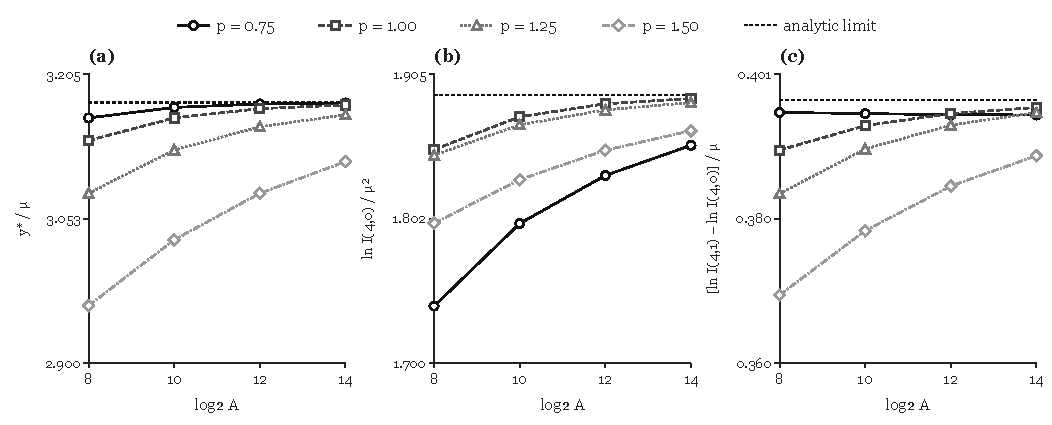
\includegraphics[width=\textwidth]{figures/heat-edge.pdf}
 \caption{Finite heat-edge diagnostic at \(s=4\).
 The four degree laws use \(m\) equal to the positive even integer
 nearest \(A^\sigma\), for \(\sigma=0.75,1,1.25,1.5\), and
 \(A=256,1024,4096,16384\).
 Panels (a)--(c) show the saddle location divided by \(\mu\),
 \(\log I_{m,A}(4,0)/\mu^2\), and
 \([\log I_{m,A}(4,1)-\log I_{m,A}(4,0)]/\mu\).
 Dashed horizontal lines are the three analytic limits. All quantities
 are dimensionless and natural logarithms are used in (b)--(c).
 Each panel has a separately enlarged vertical range. The
 \(\sigma=0.75\) tilt sequence moves slightly away from its limit on
 this finite grid; convergence is not asserted from these plotted
 values. The letter \(p\) in the figure legend denotes \(\sigma\)
 here, not the pressure or the scale parameter \(p_0\).}
 \label{fig:edge-diagnostic}
\end{figure}

The calculation uses deterministic IEEE-754 binary64
quadrature, with 40\,001 grid points for the fine calculation and
20\,001 for comparison, and a log-phase drop of 48 to truncate the
integration interval. The ancillary directory \texttt{anc/heat-edge/}
contains the plotting source, parameters, and all 16 data rows;
\texttt{plot.py --check} reproduces the numerical comparison report. The two-resolution and tail-truncation comparisons measure
stability of this finite calculation. They provide no error enclosure
for every degree and scale. The limiting assertions and the
Navier--Stokes conclusions are justified by the analytic proofs.

This figure illustrates the qualitative limits, not the
quantitative bounds or the second-kind extension. Exact algebra
checks are included in \texttt{anc/checks/}; neither is a continuum certificate.


\begingroup
\small
\setlength{\bibsep}{4pt}
\interlinepenalty=10000
\bibliographystyle{plainnat}
\bibliography{references}
\endgroup
\end{document}
